% !TeX spellcheck = en_US
\documentclass[11pt,letterpaper]{article}
%%% This file is the preamble for the Pomona Linguistics Paper Template. 
%For stacking text, used here in autosegmental diagrams
\usepackage{stackengine}

%To combine rows in tables
\usepackage{multirow}
\usepackage{multicol}
\usepackage{enumitem}
\usepackage{subcaption}

%geometry helps manage margins, among other things.
\usepackage[margin =1in]{geometry}
\usepackage{tabularx}
%used to draw the bullet below
\usepackage{graphicx}

%Gives some extra formatting options, e.g. underlining/strikeout
\usepackage{ulem}

%For putting links into papers, also helps make cross-references in the paper smart references
\usepackage[colorlinks = true,
linkcolor = blue,
urlcolor  = blue,
citecolor = blue,
anchorcolor = blue]{hyperref} %smarter cross-references, these options turn links blue

%Use package/command below to create a double-spaced document, if you want one. Uncomment BOTH the package and the command (\doublespacing) to create a doublespaced document, or leave them as is to have a single-spaced document.
\usepackage{setspace}
\onehalfspacing

%paragraph formatting
\usepackage[parfill]{parskip}
\setlength{\parindent}{20pt}
\usepackage{titlesec}

%to position tables where I want
\usepackage{float}


%Basic math symbols 
\usepackage{pifont}
\usepackage{amssymb}
%\usepackage{nath}

%%%Gives shortcuts for glossing. The use of this package is NOT explained in the Quick Reference Guide, but the documentation is on CTAN for those that are interested. MJKD finds it handy for glossing. (https://ctan.org/pkg/leipzig?lang=en)
\usepackage{leipzig}

%Tables
\usepackage{caption} %For table captions
\usepackage{booktabs} %helps format tables

%For citations and bibliography - as of 9.1.2019 we don't explain citations in this Quick Reference Guide, but Pedro Martin's tutorial does (see links in the Guide).
\usepackage{natbib}

%Fonts
\usepackage{libertine}
\setmonofont[Scale=0.8]{Courier New Bold}
\usepackage{tipa}

%highlights text with \hl{text}
\usepackage{color, soul}

%%% 
% Customizing appearance of to-do notes
\usepackage[color=blue!20, bordercolor=blue]{todonotes}
\usepackage{algorithm}
\usepackage{algpseudocode}

\usepackage{verbatim} % for verbatim text
\usepackage{adjustbox} % for adjusting row height
\usepackage{array} % for centering text vertically in cells

%To combine rows in tables
\usepackage{multirow}
\usepackage{graphicx}
\usepackage{setspace}
%\doublespacing 


%Drawing Syntax Trees
\usepackage[linguistics]{forest}

%This specifies some formatting for the forest trees to make them nicer to look at
\forestset{
	asr/.style={
		for tree={
			align=center,
			parent anchor=south,
			%   child anchor=north,
			s sep=4mm,
			l sep=6mm
		}
	},
	strike/.style={
		edge label={
			node[midway, sloped, rotate=90] {=}
		}
	}
}

%These are useful for some of the details of arrows and other parts of syntax diagrams
\usetikzlibrary{positioning} %I've included this for the sake of making figures!
\usepackage{pstricks}
\usepackage{pst-node}



%% For numbered and glossed examples %%
\usepackage{gb4e}



\usepackage{tikz}

\newcommand{\circled}[1]{\begin{tikzpicture}[baseline=(word.base)]
	\node[draw, rounded corners, text height=8pt, text depth=2pt, inner sep=2pt, outer sep=0pt, use as bounding box] (word) {#1};
\end{tikzpicture}
}

\tikzset{
	state/.style={circle, draw, minimum size=20pt, inner sep=5pt}
}


%%%%%%%%%%%%%%%%%%%%%%%%%%%%%%%%%%%%%%%%%%%%%%%%%%%%%%%%%%%%
%%%%%%%%%%%%%%%%%%%%%%%%%%%%%%%%%%%%%%%%%%%%%%%%%%%%%%%%%%%%

% Useful Ling Shortcuts

\RequirePackage{leipzig}
%\RequirePackage{mathtools} % for \mathrlap

% % % Shortcuts  (borrowed from JZ, I'm still unsure exactly what xspace requires)
\RequirePackage{xspace}
\xspaceaddexceptions{]\}}

%This makes the \emptyset command be a nicer one
\let\oldemptyset\emptyset
\let\emptyset\varnothing
\newcommand{\nothing}{$\emptyset$}

%Not all of these are explained in the Quick Reference Guide, but they are here bc they are relevant to some of our students.
\newcommand{\1}{\rlap{$'$}\xspace}
\newcommand{\0}{\rlap{\textsuperscript{$ˆ{\circ}$}}\xspace}
\newcommand{\Lb}[1]{$\text{[}_{\text{#1}}$ } %A more convenient left bracket
\newcommand{\Rb}[1]{$\text{]}_{\text{#1}}$ } %A more convenient left bracket
\newcommand{\gap}{\underline{\hspace{1.2em}}}
\newcommand{\vP}{\emph{v}P}
\newcommand{\lilv}{\emph{v}}
\newcommand{\Abar}{A$'$-} %A more convenient A-bar notation
\newcommand{\ph}{$\varphi$\xspace} %A more convenient phi
\newcommand{\pro}{\emph{pro}\xspace}
\newcommand{\subs}[1]{\textsubscript{#1}} %A more convenient subscript
%\newcommand{\hd}{$^{\circ}$\xspace} %Symbol for printing head / degree symbol
\newcommand{\spells}{$\Longleftrightarrow$} %spellout arrow for morph spellout rules
\newcommand{\tr}[1]{\textit{t}\textsubscript{\textit{#1}}} %easy traces with subscript
\newcommand{\supers}[1]{\textsuperscript{#1}}
\newcommand{\type}[1]{\ensuremath{\langle{#1}\rangle}}% Type brackets for type-theory 	 ... \type{e,\type{s,t}}, from linguistics package			
\newcommand{\nl}{\ensuremath{\varnothing}}	  % =null; Null symbol ... \nl  (\null is already used) % Requires amssymb package, or a class that calls it %From Linguistics package

%This creates the command \bigcdot which is nice as a bullet for the conventional implicature formalism. Adapted from here: https://tex.stackexchange.com/questions/235118/making-a-thicker-cdot-for-dot-product-that-is-thinner-than-bullet
\makeatletter
\newcommand*\bigcdot{\mathpalette\bigcdot@{1}}
\newcommand*\bigcdot@[2]{\mathbin{\vcenter{\hbox{\scalebox{#2}{$\m@th#1\bullet$}}}}}
\makeatother



%%%%%%%%%%%%%%%%%%%%%%%%%%%%%%%%%%%%%%%%%%%%%%%%%%%%%%%%%%%%
%%%%%%%%%%%%%%%%%%%%%%%%%%%%%%%%%%%%%%%%%%%%%%%%%%%%%%%%%%%%

%A couple of packages that seemed to prefer being called toward the end of the preamble

%This package provides macros for typesetting SPE-style phonological rules.
\usepackage{phonrule}

%For using Greek letters outside of math mode.
\usepackage{textgreek}


%Random, lets us use the XeLaTeX logo. Not important to the template at all.
\usepackage{metalogo}

%The packages and tikz libraries below are used to generate the arrows on forest trees and linear diagrams that are explained in our Arrows explainer. https://www.overleaf.com/latex/templates/arrows-for-syntax-diagrams-with-forest/xjyvcszgcspv

\usetikzlibrary{positioning} %does something for the positioning of arrows and I can't remember what
\usetikzlibrary{arrows,arrows.meta} %gives extra details for arrows (specifically, the tips of arrows)
\usepackage{pstricks} %for horizontal arrows in linear diagrams
\usepackage{pst-node} %for placing nodes in horizontal arrow diagrams

\usepackage{forest}
\title{Learning Tonotactic Patterns over Autosegmental Representations}
\author{Han Li}
\date{\today}

\begin{document}
 
	\maketitle
	
\begin{abstract}
	Autosegmental theory \citep{goldsmith1976autosegmental} proposes that tone should be represented in a tier separate from segmental tier, and both tiers are linked through associations governed  by wellformedness conditions. Tonotactic patterns can be easily expressed over autosegmental representations (ARs). This paper is the first to show how tonotactic patterns can be learned over ARs. It uses the bottom-up learning algorithm proposed by \cite{chandleeLearningPartiallyOrdered2019}, which captures the most general constraints that adequately cover a given finite set of positive data  with model-theoretic representations. An experimental case study was conducted using tonal data from Hausa, a Chadic language mainly spoken in West Africa. The experiment revealed 26 distinct ARs among 664 surface-true Hausa words, and identified 7 AR structures (syllable number \(\leq 3 \) , tone number \(\leq 3\)) missing from the data, which constitutes the constraints in the tonal grammar. The computationally discovered constraints either match ones previously proposed or better\hl{provide more explicit contexts}. Additionally, patterns not previously reported were also identified by the algorithm. The paper demonstrates the feasibility and efficiency of ARs as a possible representation for grammar inference.
\end{abstract}

\setlength\parskip{3pt}
\section{Introduction}

Tonal phonology differs from segmental phonology due to the nonlinear nature of tonotactic patterns. For wellformedness of tonotactic patterns, tonal units (such as H and L) and their associations with timing units need to be taken into consideration. This characteristic is captured in Autosegmental Theory \citep{goldsmith1976autosegmental}, which proposes that tone should be represented on a tier separate from the segmental tier, and both tiers are linked through associations regulated by a set of wellformedness conditions. Subsequently, autosegmental theory has demonstrated distinct advantages in representing prevalent tonotactic patterns \citep{hyman2011tone}, for which linear theories struggle to formalize \citep{odden1994adjacency}.


Despite the importance of ARs in tonal phonology,there is little work on using them in learning. This paper offers the first attempt at learning tonotactic patterns over ARs instead of string representations. Distinct ARs are represented by model-theoretic representations which can fully capture the unique internal AR structures. The paper focuses on three major questions concerning tonotactic learning: why tonotactic patterns are preferably learned with ARs; whether any algorithm can learn the tonotactic grammar of the language, and what tonotactic patterns can be found by the algorithm and what they reveal to us. Using a case study from Hausa, I show that a bottom-up learning algorithm \citep{chandleeLearningPartiallyOrdered2019} successfully captures the tonotactic constraints over autosegmental representations in the language. Further analysis reveals that among these constraints, not only are there those previously attested in linguistic analysis but also there are those never reported before which have been discovered.
 

To be more specific, consider one commonly discussed example of tonal mapping from the HL and LH melody in Hausa and Mende \citep{jardineLocalNatureToneassociation2017, zoll2003optimal}. The two languages form a ``mirror image'' of each other. They first differ in their contour formation: in Mende, rising tones are permitted on monosyllabic words but they are forbidden in Hausa. Secondly, when it comes to the 2-tone melody mapping onto a trisyllabic word, Mende and Hausa have distinct surface forms: a HL becomes HLL in Mende trisyllabic words but HHL in Hausa, and LH becomes LLH in Mende but LHH in Hausa.\footnote{In this paper, when two identical tones occur adjacent to each other, I will follow the tonal transcription method commonly used by Africanists, where "HH" represents two adjacent syllables both having a high tone \citep{Leben, Newmanbook, zoll2003optimal}. This shorthand notation does not necessarily indicate a violation of the Obligatory Contour Principle in Autosegmental Theory \citep{goldsmith1976autosegmental}. The same rationale applies to the "HHL" (two H-toned syllables followed by a L-toned syllable), "LHH" (a L-toned syllable followed by two H-toned syllables) and similar notations used elsewhere. Concerning ARs, \citet{jardine-heinz-2015-concatenation} showed how to convert such representations into ARs that obey the OCP.} Furthermore, monosyllabic \texttoptiebar{LH} are acceptable in Mende yet forbidden in Hausa. These patterns can be represented easily with ARs as shown in Table \ref{tab:2langauges}.
\begin{multicols}{2}
\ea  Mende\\ \noindent
\begin{tabular}{llll}
	HL & mbû (\texttoptiebar{HL}) & pélè (HL) & félàmà (HLL)  \\
	LH & mbǎ (\texttoptiebar{LH}) & nìká (LH) & lèlèmá  (LLH)
\end{tabular}
    \z
\ea Hausa\\
 \noindent
\begin{tabular}{lll}
	bût (\texttoptiebar{HL}) & wátà:(HL) & láhádì  	(HHL)  \\
	--                       & ìná 	(LH) & àshá:ná: (LHH)
\end{tabular}
\z
\end{multicols}

\begin{table}[!htbp]
    \centering
\begin{tabular}{c|cc|c} \hline 
Wellformed language/pattern & LH& HL&contours\\ \hline  
Mende&
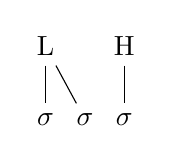
\begin{tikzpicture}
    \node (t1) at (1,1) {L};
    \node (t2) at (2,1) {H};
    \node[anchor=base] (c1) at (1,0) {$\sigma$};
    \node[anchor=base] (c2) at (1.5,0) {$\sigma$};
    \node[anchor=base] (c3) at (2,0) {$\sigma$};
    \draw (t1) -- (c1);
    \draw (t1) -- (c2);
    \draw (t2) -- (c3);
\end{tikzpicture} &
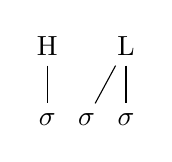
\begin{tikzpicture}
    \node (t1) at (1,1) {H};
    \node (t2) at (2,1) {L};
    \node[anchor=base] (c1) at (1,0) {$\sigma$};
    \node[anchor=base] (c2) at (1.5,0) {$\sigma$};
    \node[anchor=base] (c3) at (2,0) {$\sigma$};
    \draw (t1) -- (c1);
    \draw (t2) -- (c2);
    \draw (t2) -- (c3);
\end{tikzpicture}&
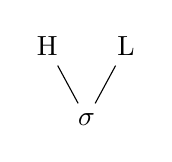
\begin{tikzpicture}
    \node (t1) at (1,1) {H};
    \node (t2) at (2,1) {L};
    \node[anchor=base] (c1) at (1.5,0) {$\sigma$};
    \draw (t1) -- (c1);
    \draw (t2) -- (c1);
\end{tikzpicture} 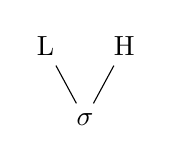
\begin{tikzpicture}
    \node (t1) at (1,1) {L};
    \node (t2) at (2,1) {H};
    \node[anchor=base] (c1) at (1.5,0) {$\sigma$};
    \draw (t1) -- (c1);
    \draw (t2) -- (c1);
\end{tikzpicture} 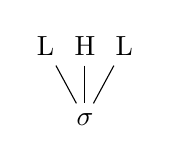
\begin{tikzpicture}
    \node (t1) at (1,1) {L};\node (t3) at (2,1) {L};
    \node (t2) at (1.5,1) {H};
    \node[anchor=base] (c1) at (1.5,0) {$\sigma$};
    \draw (t1) -- (c1);
    \draw (t2) -- (c1); \draw (t3) -- (c1);
\end{tikzpicture}\\ \hline
Hausa &
    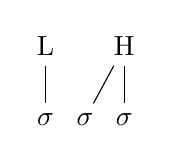
\begin{tikzpicture}
    \node (t1) at (1,1) {L};
    \node (t2) at (2,1) {H};
    \node[anchor=base] (c1) at (1,0) {$\sigma$};
    \node[anchor=base] (c2) at (1.5,0) {$\sigma$};
    \node[anchor=base] (c3) at (2,0) {$\sigma$};
    \draw (t1) -- (c1);
    \draw (t2) -- (c2);
    \draw (t2) -- (c3);
\end{tikzpicture}&
    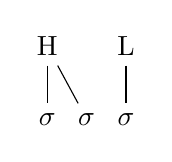
\begin{tikzpicture}
    \node (t1) at (1,1) {H};
    \node (t2) at (2,1) {L};
    \node[anchor=base] (c1) at (1,0) {$\sigma$};
    \node[anchor=base] (c2) at (1.5,0) {$\sigma$};
    \node[anchor=base] (c3) at (2,0) {$\sigma$};
    \draw (t1) -- (c1);
    \draw (t1) -- (c2);
    \draw (t2) -- (c3);
\end{tikzpicture} &
    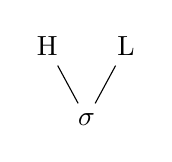
\begin{tikzpicture}
    \node (t1) at (1,1) {H};
    \node (t2) at (2,1) {L};
    \node[anchor=base] (c1) at (1.5,0) {$\sigma$};
    \draw (t1) -- (c1);
    \draw (t2) -- (c1);
\end{tikzpicture}\\ \hline  
\end{tabular}
\caption{2-tone trisyllabic forms and contours in Hausa and Mende}
\label{tab:2langauges}
\end{table}

\cite{jardineLocalNatureToneassociation2017} explains how these tonotactic patterns over ARs can be expressed as graphs (see also \cite{coleman1991no, jardine-heinz-2015-concatenation}). First, there is a set of labeled nodes representing elements from the two tiers of information in ARs: one from the tonal tier and the other from the TBU tier. On each tier, the fixed order of the elements is depicted with directed edges. Between two tiers, undirected edges link elements corresponding to association lines in ARs. As shown in Figure \ref{fig:notHLL}, labeled nodes are represented by circles with labels inside them; directed edges are arrows with heads; undirected edges are represented with lines between two tiers. One can see each AR and its graph is identical in terms of their tonal sequence, TBU numbers, and association lines. Hence, we can define a wellformed AR as one does not contain any graph or connected pieces of a graph (known as subfactors) that is considered a constraint in the grammar. For example, in Hausa, the absence of a monosyllabic rising tone can be understood as the language forbidding the structure where two tonal nodes, a L followed by a H, connect to the same TBU node on the timing tier as in Figure \ref{cons:lh1}. If any AR contains (\ref{cons:lh1}), for instance as (\ref{cons:lh2}) or (\ref{cons:lh3}) does, it will be identified illicit as well. 

More formally, if Grammar $G$ is the set of constraints
 in the language, such that $G = \{r_1, r_2, \ldots, r_n\}$, a wellformed structure is one that contains no forbidden subfactors, or equivalently, the one satisfies the conjunction of negative literals: $\lnot r_1 \land \lnot r_2 \land \lnot r_3 \land \ldots \land \lnot r_n$ \citep{jardineLocalNatureToneassociation2017, rogers2019extracting}. 

\begin{figure}[ht]%\centering
	\begin{multicols}{3}
		
		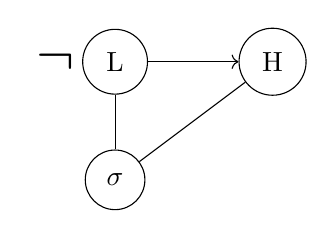
\begin{tikzpicture} 
			\node [] (s1) at (-0.75,1.5) {\huge \textbf{$\neg$}};
			\node [state] (s1) at (0,0) {$\sigma$};
			\node [state] (t1) at (0,1.5) {L};
			\node [state] (t2) at (2,1.5) {H};
			\draw [->] (t1) to (t2);
			\draw (t1) to (s1);
			\draw (t2) to (s1);
		\end{tikzpicture} 
		\subcaption{*$\check{\sigma}$}
		\label{cons:lh1}
	 
		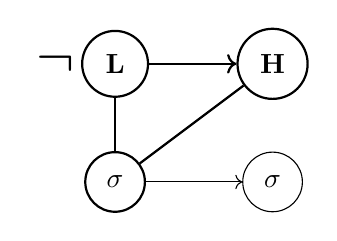
\begin{tikzpicture} 
			\node [] (s1) at (-0.75,1.5) {\huge \textbf{$\neg$}};
			\node [thick, state] (s1) at (0,0) {\textbf{$\sigma$}};
			\node [state] (s2) at (2,0) {$\sigma$};
			\node [thick, state]  (t1) at (0,1.5) {\textbf{L}};
			\node [thick, state]  (t2) at (2,1.5) {\textbf{H}};
			\draw [thick, ->] (t1) to (t2);
			\draw [thick] (t1) to (s1);
			\draw [thick] (t2) to (s1);
			\draw [->] (s1) to (s2);
		\end{tikzpicture} 
		\subcaption{*$\check{\sigma}\sigma$}
		\label{cons:lh2}
	
		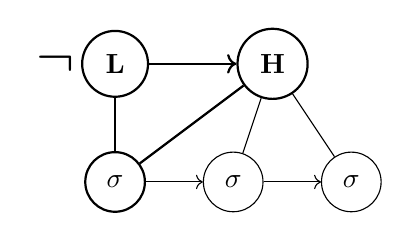
\begin{tikzpicture} 
			\node [] (s1) at (-0.75,1.5) {\huge \textbf{$\neg$}};
			\node [thick, state] (s1) at (0,0) {\textbf{$\sigma$}};
			\node [state] (s2) at (1.5,0) {$\sigma$};
			\node [state] (s3) at (3,0) {$\sigma$};
			\node [thick, state]  (t1) at (0,1.5) {\textbf{L}};
			\node [thick, state]  (t2) at (2,1.5) {\textbf{H}};
			\draw [thick, ->] (t1) to (t2);
			\draw [thick] (t1) to (s1);
			\draw [thick] (t2) to (s1);
			\draw (t2) to (s2);
			\draw (t2) to (s3);
			\draw [->] (s1) to (s2);
			\draw [->] (s2) to (s3);
		\end{tikzpicture} 
		\subcaption{*$\check{\sigma}\acute{\sigma}\acute{\sigma}$}
		\label{cons:lh3}
	
	\end{multicols}
	\caption{A forbidden structure *LH}
	\label{fig:notHLL}
\end{figure}

Naturally, the next major question would be how these constraints can be learned computationally. In other words, is it possible to learn the set of constraints from example words, and thus capture the Grammar of the language? \cite{chandleeLearningPartiallyOrdered2019} introduce a bottom-up learning algorithm which is capable of discovering the most general forbidden subfactors represented in model-theoretic forms in a language, given a finite set of examples (known as positive data). I tested this algorithm using tonotactic data from Hausa, a Chadic language spoken in West Africa, as a case study. The data were represented over ARs using a model-theoretic approach. The aim was to compare the matches between computationally detected constraints and linguistically attested constraints. It is hoped that this will not only provide more insights into tonotactic patterns under computational contexts but also show the efficacy of ARs for tonal language data. 

This paper is structured as follows. In Section 2, I will introduce key concepts in autosegmental theory and emphasize the advantages of representing tones over ARs rather than linear phonology. Section 3 will present the preliminaries in formal language and model theory. Building on the foundations laid in Section 3, Section 4 will provide a detailed description of the algorithm implementation over AR models. In Section 5, I will introduce the Hausa data used in the case study and explain how string are converted into ARs to fit algorithm implementation. Section 6 will discuss the results of the experiment, followed by the conclusion and future questions in Section 7.


\section{Autosegmental and String Representation }
One important question before moving onto any learning problems is that why should autosegmental representations be favored over string representations or features in tonal phonology. In this section, I will review arguments supporting that ARs offer advantages over linear theories for tonal phonology. Three commonly discussed tonal phenomenon (reviewed in details along with more arguments in \citet{oddenbook}) are relevant to tonotactic patterns as well as computational grammar inference:
\begin{enumerate}
\item Contour formation: complex tones emerge as a result of readjusting tonal units with timing units in autosegmental theory rather than changing feature values;
\item Melodic tonal restriction: languages have limited number of tonal sequences which are independent from their segmental content;
\item Non-local or ``across-the-board'' patterns: one tone unit can operate over multiple segments; 

\end{enumerate}

These arguments support AR as a better and more explicit representation of tones. 


\subsection{Complex tones over ARs}
First, contours typically form when two contrastive tones occupy the same tone-bearing unit, resulting in a complex tone formed in the original sequential order. With linear representations, tones are either represented with tone labels (H, L, M, F, R) or with features (H as [+H], L as [-H],  R as [-H, +contour] and F as [+H, +contour]), which are treated as properties of the segments. Derivational contours are typically formalized as changes in labels or feature values as in (\ref{tonerules}) and (\ref{featrule}), where contour tones [+contour] emerge as a result of two opposing tone values are adjacent.

\begin{multicols}{2}
\ea \label{tonerules}
\phonr{H}{F}{L}\\
\phonr{L}{R}{H}\z
\ea \label{featrule}
\phonr{[+High]}{[+contour]}{[-High]}\\
\phonr{[-High]}{[+contour]}{[+High]}\z
\end{multicols}


However, this formalization approach leads to undergeneralization and overgeneralization. The feature system struggles to generalize processes when H becomes R before L or F; or when L becomes F before H or R. In these two cases, natural classes are needed to incorporate \{L, F\} and \{H, R\}, which is impossible since no set of feature-values picks out the two tones in each group. On the other hand, within the feature system, patterns such as those in (\ref{overg}) are predicted, but they are unattested in any tonal languages discovered so far.

\begin{multicols}{2}
	\noindent
	\begin{minipage}[t]{1.2\linewidth}
		\centering
		\ea  \label{underg}
		Undergeneralization\\
		^?\phonr{[+H]}{[+contour]}{\{[-H],[+H, +contour]\}} \\
		^?\phonr{[-H]}{[+contour]}{\{[+H],[-H, +contour]\}}
		\z 
	\end{minipage}
	\hfill
	\begin{minipage}[t]{1\linewidth}
		\centering
		\ea \label{overg}
		Overgeneralization\\
		*\phonl{[+H]}{[+contour]}{[-H]}\\
		*\phonl{[-H]}{[+contour]}{[+H]}
		\z
	\end{minipage}
\end{multicols}

Furthermore, the linear theory shows more difficulty with convex (FR) and concave (RF) tones, which only increases the tonal inventory. Mongo \citep{odden1994adjacency} has the three-tone contours FR and RF. If these tones are viewed as inseparable and inherent tonal types in the inventory, the inventory will increase from 2 (H and L) to 6 (H, L, F, R, FR, RF). If so, one could expect 36 combinations for a disyllabic word, and 216 for a trisyllabic words.

\begin{table}[ht]
\ea Mongo

\begin{tabular}{llll}
		bàlóngá  b\v akáé                    & $\rightarrow$ & bàlóng\textfallrise{a} káé          & H + R $\rightarrow$ FR \\
		fàkàlà   \^ \textopeno tswà          & $\rightarrow$ & fàkàl\textrisefall{\textopeno} tswà & L + F $\rightarrow$ RF \\
		b\v ankò  b\v am\v \textopeno        & $\rightarrow$ & b\v ank\v am\v \textopeno           & L + R $\rightarrow$ R  \\
		\v \textopeno m\v \textopeno \  êmbè & $\rightarrow$ & \v \textopeno m\textrisefall{e} mbè & R + F $\rightarrow$ RF
	\end{tabular}
	\label{ex:mongo}
\z
\end{table}

Autosegmental phonology, on the other hand, views tonal processes not as arbitrary changes in feature values, but rather as adjustments or re-associations of tones and timing units. From this perspective, contour tones emerge as a result of two tones associating with a single tone-bearing unit. This significantly reduces the necessity for a large inventory of units which integrate tones with segmental content, and provides a more straightforward analysis of complex tone preservation processes, even as observed in Mongo. In (\ref{ar.mongo}), no new tonal types are introduced into the inventory nor is there any change in the melody (from L-HL to LHL). Instead, there are two changes: the deletion of vowel a in the segment tier and the dissociation of \textit{a} from L,  which then spreads onto the following segment. As a result, the vowel \textit{\textopeno} is associated to 3 tones LHL which corresponding to RF in Ex (\ref{ar.mongo}).

\ea \label{ar.mongo}
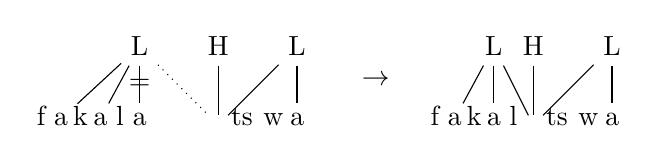
\begin{tikzpicture}
	%tone tier (4 tones)
	\node (t1) at (2.25,1) {L};
	\node (t4) at (3.25,1) {H};
	\node (t5) at (4.25,1) {L};
	\node[anchor=base] (c1) at (1,0) {f} ;
	\node[anchor=base] (v1) at (1.25,0) {a} ;
	\node[anchor=base] (c2) at (1.5,0) {k} ;
	\node[anchor=base] (v2) at (1.75,0) {a} ;
	\node[anchor=base] (c3) at (2,0) {l} ;
	\node[anchor=base] (v3) at (2.25,0) {a} ;
	%\node[anchor=base] (add) at (2.75,0.5) {+} ;
	\node[anchor=base] (v4) at (3.25,0) {\textopeno} ;
	\node[anchor=base] (c4) at (3.55,0) {ts} ;
	\node[anchor=base] (c5) at (3.95,0) {w} ;
	\node[anchor=base] (v5) at (4.25,0) {a} ;
	\node[anchor=base] (to) at (5.25,0.5) {$\rightarrow$} ;
	\draw (t1) -- (v1);
	\draw (t1) -- (v2);
	\draw (t1) -- (v3)	node[midway, sloped, rotate=90] {=};
	\draw (t4) -- (v4);
	\draw (t5) -- (v4);
	\draw [dotted] (t1) --(v4);
	\draw (t5) -- (v5);
	
	\node (srt1) at (6.75,1) {L};
	\node (srt2) at (7.25,1) {H};
	\node (srt3) at (8.25,1) {L};

	\node[anchor=base] (sc1) at (6,0) {f} ;
	\node[anchor=base] (sv1) at (6.25,0) {a} ;
	\node[anchor=base] (sc2) at (6.5,0) {k} ;
	\node[anchor=base] (sv2) at (6.75,0) {a} ;
	\node[anchor=base] (sc3) at (7,0) {l} ;
	\node[anchor=base] (sv3) at (7.25,0) {\textopeno} ;
	\node[anchor=base] (sc4) at (7.55,0) {ts} ;
	\node[anchor=base] (sc5) at (7.95,0) {w} ;
	\node[anchor=base] (sv5) at (8.25,0) {a} ;
	
	\draw (srt1) -- (sv1);
	\draw (srt1) -- (sv2);
	\draw (srt1) -- (sv3);
	\draw (srt2) -- (sv3);
	\draw (srt3) -- (sv3);
	\draw (srt3) -- (sv5);	
\end{tikzpicture}
\z
\subsection{Melodic Tonal Restriction}
Many languages have been found to have a fixed set of melodies that ``must be abstracted away from the the TBUs on which they are realized'' \citep{hyman2011tone}.\footnote{There are languages where tonal melodies are not highly restricted such as Cantonese and Mandarin Chinese. They can be viewed as ``syllable-tone'' languages where tones do not changes when morphemes are combined together \citep{yip2002tone}. Even for these languages, \cite{sy1967phonological} pointed out the domain of tones applies over the entire voiced portion of syllables and the tone quality is irrelevant to the nature of the segment bearing the tone, and thus tone features need to be differentiated from segmental features.} In other words, there is a limited number of tonal combinations over phrases or words that a language can have. Mende is an often-cited example of this melodic tonal restriction. The language has 2 contrast tones: H and L while HL combines to F, LH to R, and LHL to RF. A trisyllablic word could therefore have \(5*5*5=125\) possible tonal combinations. However, irrespective of the syllable number, Mende only have five tonal melodies: H, L, HL, LH, and LHL. \citep{leben2017tone,oddenbook,hyman2011tone}.

\begin{table}[hb]
	\centering
	\begin{tabular}{lllll}
		\toprule
		No. & Melody Pattern & Monosyllabic & Disyllablic & Trisyllabic\\
		\midrule
		1. & /H/ & k\'\textopeno & k\'\textopeno-má &háwámá \\
		2. & /L/ & kp\`a & b\`ɛl\`ɛ & b\`ɛl\`ɛ-mà\\
		3. & /HL/ & mbû & mbú-mà & félàmà\\
		4. & /LH/ & mbǎ & mbà-má& ndàvúlá\\
		5. & /LHL/ & mbã& nyàhâ & nyàhá-mà \\
		\bottomrule
	\end{tabular}
	\caption{Mende Tone Patterns \citep[p.294]{oddenbook}}
	\label{tab:mende}
\end{table}

The same case also applies to Kukuya, where Paulian (1975, cited from \citet{hyman2011tone}) recognized same five tonal melodies that can be predicted to map onto stems of different lengths. Besides, in Kpelle, the fix tonal meldoies are /H,L,HL,M, MHL/.\footnote{\citet[p.492]{hyman2011tone} mentioned the M melody has an underlying form of /LH/ which result in Kpelle having the same tonal patterns as Mende.} These examples indicate that if tones are viewed as a segmental property, the constraints accounting for them will be more complex. Instead, the restrictions can be explained by stating that there are only five patterns of H and L combinations on the tonal tier of an AR, but they are linked to different lengths of TBUs.

\subsection{Non-local tonal patterns}
It has also been argued that ARs are favored in tonal phonology because they easily describe non-local tonal patterns which are very common among tonal languages \citep{oddenbook}. By non-local pattern it refers to the cases where a tone triggers a change that does not exclusively apply to its local neighbors but all elements in the target domain. One example is the Shona noun compound \citep{odden1994adjacency}. If the initial tone of the noun stem (leftmost column in Example \ref{ex:shona}) is a H tone, the prefix \textit{né, sé, ché} will trigger a series of L tone to change into H (\ref{ex:shona}b and \ref{ex:shona}c) until another L tone is present to block the spreading (\ref{ex:shona}d). 


\ea \label{ex:shona}
\begin{tabular}{lllll}
\textbf{N}     & \textbf{with N} & \textbf{like N} & \textbf{of N}   &  \textbf{gloss of N}           \\
a. mùrúmé      & né-mùrúmé       & sé-mùrúmé       & ché-mùrúmé      & ``man"        \\
b. mbúndúdzí   & né-mbùndùdzì    & sé-mbùndùdzì    & ché-mbùndùdzì   & ``army worms" \\
c. hákátà      & né-hákátà       & sé-hákátà       & ché-hákátà      & ``bones"      \\
d. bénzíbvùnzá & né-bènzìbvùnzá  & sé-bènzìbvùnzá  & ché-bènzìbvùnzá & ``fool"
\end{tabular}
\z

A rule could be formalized to account for this change: \phonl{[+H] } {[-H]} {\{\textit{sé,né,shé}\}}. This will cause the wrong surface forms such as *\textbf{né-mbù}ndúdzí,  *\textbf{né-hà}kátà and *\textbf{né-bèn}zíbvùnzá due to the fact that the rule will only apply to the first element right next to the H-toned prefix. To accurately capture the rule, a formula needs to capture a long-distance dependency that will apply to every element within the target domain as shown in (\ref{longdistone}).
\ea \label{longdistone}
\phonb{H}{L}{H}{(L)}\\
\phonl{HH}{LL}{H}{(L)}\\
$\ldots$\\
\phonb{H^n}{L^n}{H}{(L)}
\z

The autosegmental analysis provides a more straightforward explanation, as it accounts for the lowering phenomenon exclusively affecting the initial H tone, which may be associated with multiple syllables simultaneously. 


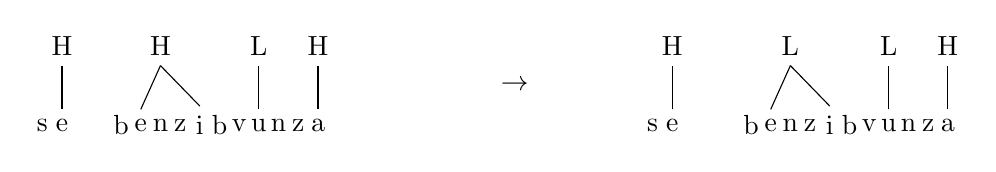
\begin{tikzpicture}
	% syllable nodes
	\node (s) at (-1,0) {s};
	\node (es) at (-0.75,0) {e};
	\node (h) at (-0.75,1) {H};
	\draw (es.north) -- (h.south);
	
	
	\node (b) at (0,0) {b};
	\node (e) at (0.25,0) {e};
	\node (n) at (0.5,0) {n};
	\node (z) at (.75,0) {z};
	\node (i) at (1,0) {i};
	\node (b2) at (1.25,0) {b};
	\node (v) at (1.5,0) {v};
	\node (u) at (1.75,0) {u};
	\node (n2) at (2,0) {n};
	\node (z2) at (2.25,0) {z};
	\node (a) at (2.5,0) {a};
	% tone nodesx
	\node (h1) at (0.5,1) {H};
	\node (l) at (1.75,1) {L};
	\node (h3) at (2.5,1) {H};
	% linking lines
	\draw (e.north) -- (h1.south);
	\draw (i.north) -- (h1.south);
	\draw (u.north) -- (l.south);
	\draw (a.north) -- (h3.south);
	
	
	\node (arrow) at (5,0.5){$\rightarrow$};
	\node (ss) at (7,0) {e};
	\node (ess) at (6.75,0) {s};
	\node (hs) at (7,1) {H};
	\draw (ss.north) -- (hs.south);
	
	\node (b2) at (8,0) {b};
	\node (e2) at (8.25,0) {e};
	\node (n2) at (8.5,0) {n};
	\node (z2) at (8.75,0) {z};
	\node (i2) at (9,0) {i};
	\node (b3) at (9.25,0) {b};
	\node (v2) at (9.5,0) {v};
	\node (u2) at (9.75,0) {u};
	\node (n3) at (10,0) {n};
	\node (z3) at (10.25,0) {z};
	\node (a2) at (10.5,0) {a};
	% tone nodesx
	\node (hh1) at (8.5,1) {L};
	\node (ll) at (9.75,1) {L};
	\node (hg3) at (10.5,1) {H};
	% linking lines
	\draw (e2.north) -- (hh1.south);
	\draw (i2.north) -- (hh1.south);
	\draw (u2.north) -- (ll.south);
	\draw (a2.north) -- (hg3.south);
	
	
\end{tikzpicture}


This example demonstrates two properties that are very common in tonal phonology but less common in segmental phonology. The first one is tonal polarity, which refers to the melodic alternation between H and L tones \citep{cahill2007more, hyman1974universals, odden1994adjacency}. The second property, unboundedness, refers to the fact that the number of tone elements subject to change is unlimited as long as the contextual environment is satisfied \citep{jardineComputationallyToneDifferent2016}.


\section{Preliminaries}
\subsection{Strings and their Representations}

Informally, a string can be understood as a sequence of characters. Let $\Sigma$ be a finite alphabet of symbols and $\Sigma^*$ the set of all strings over $\Sigma$. $|w|$ indicates the length of $w \in \Sigma^*$. For two strings $w$ and $v$,  $wv$ refers to their concatenation of two strings, and for a set $L \subseteq \Sigma^*$ of strings and a string $w$, by $wL$ we denote $\{wv \mid v \in L\}$. A string $u$ is a \textit{substring} (or a \textit{factor}) of string $v$ if there are strings $x, y \in \Sigma$ such that $u = xvy$. If $u$ is of size $k$ and is a factor of $v$, then $u$ is a $k$-factor of $v$.

A string can be represented model-theoretically. Model theory provides a uniform framework for representing objects and their relations to one another. A model-theoretic representation for strings contains two parts: the Domain \( D \) and a finite set of \( n \)-ary relations \( \mathcal{R} = \{ R_1, R_2, \ldots, R_i\} \) (\citeauthor[forthcoming]{heinzdcp}). The set of relations comprise the \textit{signature} of the model. Distinct objects will have distinct model signatures to represent the unique internal structures. The signature \( \{ R_1, R_2, \ldots, R_i \} \) includes different types of relations: unary relations represent symbols in the string, and binary relations indicate either a successor relation (denoted by $\lhd$) and a precedence relation (denoted by $\prec$) to maintain the linear order of elements. In a simple example string of strings formed with from the alphabet \{a,b\}, the representation of \textit{abaa} would be \( \mathcal{M} = \{ D \mid R_a, R_b, \lhd \} \) where \( D = \{1,2,3,4\} \) indicating there are 4 elements in the string; \(R_a\) is a unary relation for the symbol \textit{a} such that \( R_a = \{1,3,4\}\); \(R_b\) is a unary relation for the symbol \textit{b} such that \(R_b = \{2\} \), and the binary successor relation \(\lhd = \{ \langle 1,2 \rangle, \langle 2, 3 \rangle, \langle 3,4 \rangle \} \) indicates the order of elements. A diagram for the model \textit{abaa} and its signature is illustrated in Figure \ref{strmodel}.



\begin{figure}[ht]
	\centering
	\begin{multicols}{2} 
		\begin{minipage}{0.5\linewidth}
			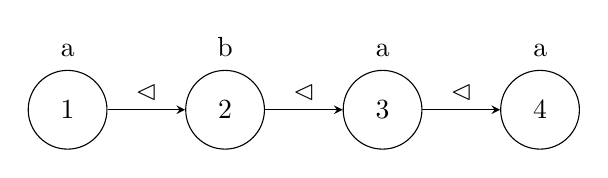
\begin{tikzpicture} [->, >=stealth, node distance=2cm, circleNode/.style={draw, circle, minimum size=1cm}]
				% Nodes
				\node[circleNode] (1) {1};
				\node[circleNode, right of=1] (2) {2};
				\node[circleNode, right of=2] (3) {3};
				\node[circleNode, right of=3] (4) {4};
				
				% Arrows with triangles
				\draw[->] (1) -- (2) node[midway, above] {$\lhd$};
				\draw[->] (2) -- (3) node[midway, above] {$\lhd$};
				\draw[->] (3) -- (4) node[midway, above] {$\lhd$};
				
				% Labels outside each circle
				\node[above=0.05cm of 1] {a};
				\node[above=0.05cm of 2] {b};
				\node[above=0.05cm of 3] {a};
				\node[above=0.05cm of 4] {a};
			\end{tikzpicture}
		\end{minipage}
		\begin{minipage}{0.6\linewidth}
			$\mathcal{M} = \{D \mid R_a, R_b, \lhd\}$\\
			$\mathcal{D} = \{1, 2, 3, 4\}$\\
			$R_a = \{1,3,4\}$ \\
			$R_b = \{2\}$ \\
			$\lhd = \{\langle 1,2\rangle, \langle 2, 3\rangle, \langle 3,4\rangle\}$ 
		\end{minipage}
	\end{multicols}
	
	\caption{String model and its signature for \textit{abaa}}
	\label{strmodel} 
\end{figure}
\subsection{ARs as Unconventional Models}

A string model can be viewed as a one-dimensional model since elements are ordered linearly on one axis. String models with successor and precedence relations have been called ``conventional" models \citep{chandleeLearningPartiallyOrdered2019,strother2017using,vu2018statistical}. Being conventional means that each element has a single and exclusive label. For example, in Figure \ref{strmodel}, the node $\{2\}$ is labeled \textit{b} and not anything else. Unlike the string model, ARs are unconventional models consisting of two strings: a tonal string and a timing string. Elements on each string are first in a successor relation and also bidirectionally connected to elements from the other string. We can refer to an AR as a bistring or a two-dimensional string. Its model signature can be constructed by initially building two string models and then combining them with association relations.

To construct the tonal string of an AR model needs a sequence of H and L alternating with each other. We could construct a successor string model with only tonal sequences as shown in Figure \ref{artonemd}. In this model, the domain \( D_t \) matches the number of tone units; two unary relations \( R_H \) and \( R_L \) refer to the H tone and L tone, respectively. Additionally, a binary relation \(\lhd_t\) represents a linear successor relation.


\begin{figure}[H]
\centering
\begin{multicols}{2} 
	\begin{minipage}{0.5\linewidth}
	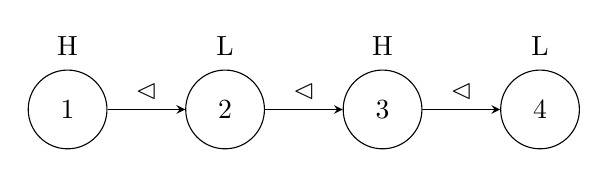
\begin{tikzpicture} [->, >=stealth, node distance=2cm, circleNode/.style={draw, circle, minimum size=1cm}]
		% Nodes
		\node[circleNode] (1) {1};
		\node[circleNode, right of=1] (2) {2};
		\node[circleNode, right of=2] (3) {3};
		\node[circleNode, right of=3] (4) {4};
		
		% Arrows with triangles
		\draw[->] (1) -- (2) node[midway, above] {$\lhd$};
		\draw[->] (2) -- (3) node[midway, above] {$\lhd$};
		\draw[->] (3) -- (4) node[midway, above] {$\lhd$};
		
		% Labels outside each circle
		\node[above=0.05cm of 1] {H};
		\node[above=0.05cm of 2] {L};
		\node[above=0.05cm of 3] {H};
		\node[above=0.05cm of 4] {L};
	\end{tikzpicture}
		\end{minipage}
	\begin{minipage}{0.6\linewidth}
		${M_t} = \{D \mid R_H, R_L, \lhd\}$\\
		${D_t} = \{1, 2, 3, 4\}$\\
		$R_H = \{1,3\}$ \\
		$R_L = \{2,4\}$ \\
		$\lhd_t = \{\langle 1,2\rangle, \langle 2, 3\rangle, \langle 3,4\rangle\}$ 
	\end{minipage}
\end{multicols}

\caption{Tonal string model \textit{HLHL } and its signature }
\label{artonemd} 
\end{figure}

Likewise, a string model for the timing string as in Figure \ref{arsylmd} can be constructed in the same fashion. The domain \( D_s \) matches the number of TBUs (syllables or moras). We will use \( R_\sigma\) to refer to TBU unary relation, which is the only element on the string. Then, TBUs are connected in a linear order. 


\begin{figure}[H]
	\centering
	\begin{multicols}{2} 
		\begin{minipage}{0.5\linewidth}
			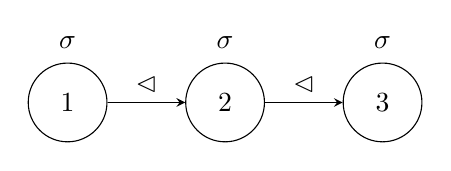
\begin{tikzpicture} [->, >=stealth, node distance=2cm, circleNode/.style={draw, circle, minimum size=1cm}]
				% Nodes
				\node[circleNode] (1) {1};
				\node[circleNode, right of=1] (2) {2};
				\node[circleNode, right of=2] (3) {3};
				
				% Arrows with triangles
				\draw[->] (1) -- (2) node[midway, above] {$\lhd$};
				\draw[->] (2) -- (3) node[midway, above] {$\lhd$};
				
				% Labels outside each circle
				\node[above=0.05cm of 1] {$\sigma$};
				\node[above=0.05cm of 2] {$\sigma$};
				\node[above=0.05cm of 3] {$\sigma$};
			\end{tikzpicture}
		\end{minipage}
		\begin{minipage}{0.6\linewidth}
			$M_s = \{D \mid R_\alpha, \lhd\}$\\
			$D_s = \{1, 2, 3\}$\\
			$R_\sigma = \{1,2,3\}$ \\
			$\lhd_s = \{\langle 1,2\rangle, \langle 2, 3\rangle\}$ 
		\end{minipage}
	\end{multicols}
	
	\caption{String model and its signature for the tonal sequence HLHL}
	\label{arsylmd} 
\end{figure}


Finally, elements from one string connect with those on the other one. Linguistically, this corresponds to the association lines in AR that indicate the arrangement of H and L with respect to the temporal order. To connect the two strings and build an AR model, a binary relation \( \alpha \) is used to represent the associations held between two strings. The signature of the combined model is the union of the signatures of the tonal string and timing string, along with the binary association relation. Specifically, the size of ${D}$ is the sum of tonal units and TBUs such that $D = \{1, 2,\ldots |D_t| + |D_s|\}$. If we renumber each distinct node, for example, with the first syllable being node 1 and the first tone node 4, we will have a model as in Figure \ref{armodel}.

\begin{figure}[ht]
	\begin{multicols}{2}
	\begin{minipage}{0.84\linewidth}
	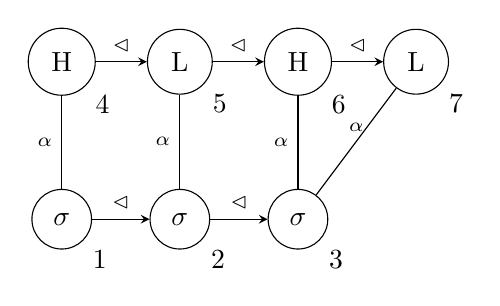
\begin{tikzpicture} [->, >=stealth, node distance=1cm, circleNode/.style={draw, circle, minimum size=1cm}]
	\node [state, label=below right:1] (s1) at (0,0) {$\sigma$};
	\node [state, label=below right:2] (s2) at (1.5,0) {$\sigma$};
	\node [state, label=below right:3] (s3) at (3,0) {$\sigma$};
	\node [state, label=below right:4] (t1) at (0,2) {H};
	\node [state, label=below right:5] (t2) at (1.5,2) {L};
	\node [state, label=below right:6] (t3) at (3,2) {H};
	\node [state, label=below right:7] (t4) at (4.5,2) {L};
	\draw [->] (t1) edge[above] node{\scriptsize{$\lhd$}} (t2);
	\draw [->] (t2) edge[above] node{\scriptsize{$\lhd$}} (t3);
	\draw [->] (t3) edge[above] node{\scriptsize{$\lhd$}} (t4);
	\draw [->] (s1) edge[above] node{\scriptsize{$\lhd$}} (s2);
	\draw [->] (s2) edge[above] node{\scriptsize{$\lhd$}} (s3);
	\draw [-] (t1) edge[left] node{\scriptsize{$\alpha$}} (s1);
	\draw [-] (t2) edge[left] node{\scriptsize{$\alpha$}} (s2);
	\draw [-] (t3) edge[left] node{\scriptsize{$\alpha$}} (s3);
	\draw [-] (t4) edge[above] node{\scriptsize{$\alpha$}} (s3);
\end{tikzpicture}
\end{minipage}
	\begin{minipage}{\linewidth}
		$M = \{D \mid R_H, R_L, R_\sigma, \lhd, \alpha \}$\\
		$D = \{1, 2, 3, 4, 5, 6, 7\}$\\
		$R_\sigma = \{1, 2, 3\}$ \\
		$R_H = \{4,6\}$ \\
		$R_L = \{5,7\}$ \\
		$\lhd = \{\langle 1,2\rangle, \langle 2, 3\rangle,  \langle 4,5\rangle,\langle 5,6\rangle,\langle 6,7\rangle \}$ \\
		$\alpha = \{\langle 1,4\rangle, \langle 4,1 \rangle, \langle 2, 5\rangle,\langle 5,2 \rangle, \langle 3, 6\rangle,\langle 6, 3\rangle,\langle 3,7\rangle,\langle 7,3\rangle\}$ 
	\end{minipage}
	\end{multicols}
	\caption{AR model for a word $\acute{\sigma}\grave{\sigma}\hat{\sigma}$ }
	\label{armodel}
\end{figure}
 
For the successor function, there are few points to mention. First, the elements in a successor relations are directed nodes, indicating a left-to-right temporal order. Secondly, the tonal string in successor relation indicates the alternation of H and L tone. No two identical tone units are allowed to be adjacent. The Obligatory Contour Principle forbids strings such as *HHL and *LLH. To expand a given AR from a successor relation, such as from (11) to (12), one can either add a tone unit which is opposite to the preceding tone on the tone tier, or add one TBU on the timing tier. 
\begin{multicols}{2}
	\ea  	
	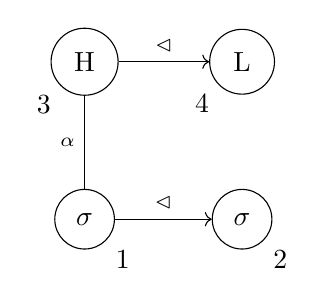
\begin{tikzpicture} 
		
		\node [state, label=below right:1] (s1) at (0,0) {$\sigma$};
		\node [state, label=below right:2] (s2) at (2,0) {$\sigma$};
		%\node [state, label=below right:3] (s3) at (4,0) {$\sigma$};
		\node [state, label=below left:3] (t1) at (0,2) {H};
		\node [state, label=below left:4] (t2) at (2,2) {L};
		\draw [->] (t1) edge[above] node{\scriptsize{$\lhd$}} (t2);
		\draw [->] (s1) edge[above] node{\scriptsize{$\lhd$}} (s2);
		%\draw [->] (s2) edge[above] node{\scriptsize{$\vartriangleright$}} (s3);
		\draw [-] (t1) edge[left] node{\scriptsize{$\alpha$}} (s1);
		%\draw [-] (t2) edge[left] node{\scriptsize{$\alpha$}} (s2);
		%\draw [-] (t2) edge[left] node{\scriptsize{$\alpha$}} (s3);
	\end{tikzpicture}
	\z
	\ea  
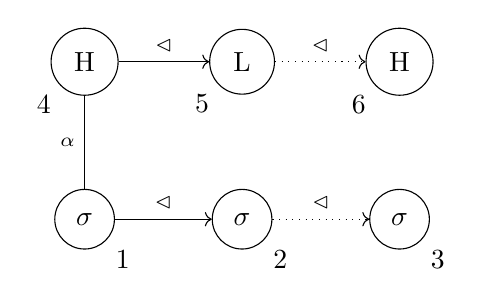
\begin{tikzpicture} 
	\node [state, label=below right:1] (s1) at (0,0) {$\sigma$};
	\node [state, label=below right:2] (s2) at (2,0) {$\sigma$};
	\node [state, label=below right:3] (s3) at (4,0) {$\sigma$};
	\node [state, label=below left:4] (t1) at (0,2) {H};
	\node [state,label=below left:5] (t2) at (2,2) {L};
	\node [state,label=below left:6] (t3) at (4,2) {H};
	\draw [->] (t1) edge[above] node{\scriptsize{$\lhd$}} (t2);
	\draw [->] (s1) edge[above] node{\scriptsize{$\lhd$}} (s2);
	\draw [->,dotted] (s2) edge[above] node{\scriptsize{$\lhd$}} (s3);
	\draw [-] (t1) edge[left] node{\scriptsize{$\alpha$}} (s1);
	\draw [->,dotted] (t2) edge[above] node{\scriptsize{$\lhd$}} (t3);
	%\draw [-] (t2) edge[left] node{\scriptsize{$\alpha$}} (s3);
\end{tikzpicture}
\z

\end{multicols}

As for the association relation, the nodes are undirected, indicating that the binary relations are doubly connected. A list of association tuples of $\langle 1, 4 \rangle, \langle 2, 5 \rangle, \langle 3, 5 \rangle$ is equivalent to  $\langle 4, 1 \rangle, \langle 5, 2 \rangle, \langle 5, 3 \rangle$. Besides, the structure allows the existence of unlinked units. For example, in (11) the L tone labeled 4 is not linked to any element in the TBU tier. In the model signature, the association relation \(\alpha = \{\langle 1,3 \rangle\}\) and does not include any of \ \{$\langle 1,4 \rangle$, $\langle 2,4 \rangle$, $\langle 4,1 \rangle$, $\langle2,4\rangle$\}. We refer the L at 4 and \(\sigma\) at 2 as \textit{floating} units. Section 4 will give more formal definition for AR expanding and floating units.

\section{Learning Autosegmental Representations}
Following \cite{jardineLocalNatureToneassociation2017}, the previous section argues that ARs can be represented in an unconventional model consisting of two strings: one on the tonal tier and the other on the syllable tier. Elements of the strings on both tiers are connected by a successor relation, while an association relation holds between the two tiers. In this section, I'll introduce a bottom-up learning algorithm proposed by \cite{chandleeLearningPartiallyOrdered2019} which was designed to learn constraints in a space of partially ordered structures. This algorithm can learn tonotactic constraints over ARs since the containment relation of ARs is also partially ordered in language.

\subsection{A Bottom-Up Learning Algorithm}
\cite{chandleeLearningPartiallyOrdered2019} discuss two directions of grammatical inference, a top-down and a bottom-up direction, the latter one is more efficient and guaranteed to find the constraints in a language. In the bottom-up learning fashion, the learner starts with the most generalized structures and move upwards to the more specific ones. Once a structure is identified missing from the positive data, the learning path moving upwards is thus discontinued and the learner will first recognize the current structure as a constraint in the language and will no longer consider its superfactors. One advantage of the algorithm is it guarantees to find the most general grammar which covers the given data. A bottom-up learning algorithm (BUFIA) is shown in Algorithm \ref{arg:bufia}.

\begin{minipage}{0.9\linewidth}
\centering
\begin{algorithm}[H]
	\caption{Bottom-Up Learning Algorithm}
	 \label{arg:bufia}
	\begin{algorithmic}
		\Require positive data $D$, empty structure $s_0$, max constraint size $k$
		\State $Q \gets \{s_0\}$ 
		\State $G \gets \emptyset$
		\State $V \gets \emptyset$
		\While{$Q \neq \emptyset$}
		\State $s \gets Q.\textsc{dequeue}()$
		\State $V \gets V \cup \{s\}$
		\If{$\exists x \in D$ such that $s \sqsubseteq x$}
		\State $S \gets \text{NextSupFact}(s)$
		\State $S' \gets \{s' \in S \,|\, |s'| \leq k \land (\lnot \exists g \in G)[g \sqsubseteq s'] \land s' \notin V\}$
		\State $Q. \textsc{enqueue}(S')$
		\Else 
		\State $G \gets G \cup \{s\}$
		\EndIf
		\EndWhile
		\State \textbf{return} $G$
	\end{algorithmic}
\end{algorithm}
\end{minipage}
\\


The algorithm initially requires three inputs: a finite size of positive data \( D \), an empty structure \( s_0 \), and a maximum constraint size \( k \). The positive data \( D \) contains a finite set of surface-true structures in the language. The empty structure \( s_0 \) is a structure that has a length of zero. The factor \( k \) limits the size of structures considered by the algorithm. Additionally, the algorithm initializes two empty sets: \( G \), representing the grammar which is empty at first and will be returned with constraints discovered by the algorithm once the learning is complete; and a set \( V \) which stores checked structures to prevent the learner from revisiting those structures that have been examined.


A queue \(Q\) is used to store structures awaiting to be checked by the algorithm. As shown in the Algorithm \ref{arg:bufia}, there are two operations related to \(Q\): \(Q\).\textsc{dequeue} and  \(Q.\)\textsc{enqueue}. The former is to take a structure \(s\) out of the queue for later checking, and the latter is to add the next structure into the \(Q\). 


Once the learning starts, BUFIA initiates from the most generalized and least complex structure, the empty structure. It then checks whether the current structure is present in the dataset. If the structure is found, the `NextSupFact' function generates its immediate superfactors which have a size $\leq k$, are not visited, and contain no structures that have been already forbidden by the grammar. The superfactors will be appended to the rear of the queue for later checking. If any structure is absent from the dataset, the algorithm adds it to the Grammar $G$ and ceases to generate its superfactors. This process repeats until the size of the structure exceeds a predetermined threshold \(k\). 

The structures added into $G$ are those missing from the positive data, indicating that the current structure is not considered as a wellformed structure but a constraint in the language. Once a structure is considered forbidden, none of its superfactors will be checked by the learner.



\subsection{Implementing BUFIA over Autosegmental Representations}
To have BUFIA learn tonotactic patterns over ARs, we need to convert the data representation into ARs and determine the measurement of a size of an AR. Here, the data in the positive sample \( D \) are represented in ARs and three factors measure its size: the length of tonal tier \(t\), the length of the syllable tier \(s\), and the number of associations formed between two tiers \(\vert \alpha\vert\). A total size \(k\) would be the sum of three factors: \(k = t+s+\vert\alpha\vert\). Following this principle, an empty AR has a length of 0 on the tonal tier, timing tier or associations in between hence its size \(k\) is 0. The partially ordered hypothesis space of ARs is shown in Figure \ref{fig:ARspace}.
\begin{figure}[ht]
	\centering
	% lattice.tex
%\documentclass{standalone}
%\usepackage{tikz}
%\usetikzlibrary{fit} % Importing the fit library
%%%% This file is the preamble for the Pomona Linguistics Paper Template. 
%For stacking text, used here in autosegmental diagrams
\usepackage{stackengine}

%To combine rows in tables
\usepackage{multirow}
\usepackage{multicol}
\usepackage{enumitem}
\usepackage{subcaption}

%geometry helps manage margins, among other things.
\usepackage[margin =1in]{geometry}
\usepackage{tabularx}
%used to draw the bullet below
\usepackage{graphicx}

%Gives some extra formatting options, e.g. underlining/strikeout
\usepackage{ulem}

%For putting links into papers, also helps make cross-references in the paper smart references
\usepackage[colorlinks = true,
linkcolor = blue,
urlcolor  = blue,
citecolor = blue,
anchorcolor = blue]{hyperref} %smarter cross-references, these options turn links blue

%Use package/command below to create a double-spaced document, if you want one. Uncomment BOTH the package and the command (\doublespacing) to create a doublespaced document, or leave them as is to have a single-spaced document.
\usepackage{setspace}
\onehalfspacing

%paragraph formatting
\usepackage[parfill]{parskip}
\setlength{\parindent}{20pt}
\usepackage{titlesec}

%to position tables where I want
\usepackage{float}


%Basic math symbols 
\usepackage{pifont}
\usepackage{amssymb}
%\usepackage{nath}

%%%Gives shortcuts for glossing. The use of this package is NOT explained in the Quick Reference Guide, but the documentation is on CTAN for those that are interested. MJKD finds it handy for glossing. (https://ctan.org/pkg/leipzig?lang=en)
\usepackage{leipzig}

%Tables
\usepackage{caption} %For table captions
\usepackage{booktabs} %helps format tables

%For citations and bibliography - as of 9.1.2019 we don't explain citations in this Quick Reference Guide, but Pedro Martin's tutorial does (see links in the Guide).
\usepackage{natbib}

%Fonts
\usepackage{libertine}
\setmonofont[Scale=0.8]{Courier New Bold}
\usepackage{tipa}

%highlights text with \hl{text}
\usepackage{color, soul}

%%% 
% Customizing appearance of to-do notes
\usepackage[color=blue!20, bordercolor=blue]{todonotes}
\usepackage{algorithm}
\usepackage{algpseudocode}

\usepackage{verbatim} % for verbatim text
\usepackage{adjustbox} % for adjusting row height
\usepackage{array} % for centering text vertically in cells

%To combine rows in tables
\usepackage{multirow}
\usepackage{graphicx}
\usepackage{setspace}
%\doublespacing 


%Drawing Syntax Trees
\usepackage[linguistics]{forest}

%This specifies some formatting for the forest trees to make them nicer to look at
\forestset{
	asr/.style={
		for tree={
			align=center,
			parent anchor=south,
			%   child anchor=north,
			s sep=4mm,
			l sep=6mm
		}
	},
	strike/.style={
		edge label={
			node[midway, sloped, rotate=90] {=}
		}
	}
}

%These are useful for some of the details of arrows and other parts of syntax diagrams
\usetikzlibrary{positioning} %I've included this for the sake of making figures!
\usepackage{pstricks}
\usepackage{pst-node}



%% For numbered and glossed examples %%
\usepackage{gb4e}



\usepackage{tikz}

\newcommand{\circled}[1]{\begin{tikzpicture}[baseline=(word.base)]
	\node[draw, rounded corners, text height=8pt, text depth=2pt, inner sep=2pt, outer sep=0pt, use as bounding box] (word) {#1};
\end{tikzpicture}
}

\tikzset{
	state/.style={circle, draw, minimum size=20pt, inner sep=5pt}
}


%%%%%%%%%%%%%%%%%%%%%%%%%%%%%%%%%%%%%%%%%%%%%%%%%%%%%%%%%%%%
%%%%%%%%%%%%%%%%%%%%%%%%%%%%%%%%%%%%%%%%%%%%%%%%%%%%%%%%%%%%

% Useful Ling Shortcuts

\RequirePackage{leipzig}
%\RequirePackage{mathtools} % for \mathrlap

% % % Shortcuts  (borrowed from JZ, I'm still unsure exactly what xspace requires)
\RequirePackage{xspace}
\xspaceaddexceptions{]\}}

%This makes the \emptyset command be a nicer one
\let\oldemptyset\emptyset
\let\emptyset\varnothing
\newcommand{\nothing}{$\emptyset$}

%Not all of these are explained in the Quick Reference Guide, but they are here bc they are relevant to some of our students.
\newcommand{\1}{\rlap{$'$}\xspace}
\newcommand{\0}{\rlap{\textsuperscript{$ˆ{\circ}$}}\xspace}
\newcommand{\Lb}[1]{$\text{[}_{\text{#1}}$ } %A more convenient left bracket
\newcommand{\Rb}[1]{$\text{]}_{\text{#1}}$ } %A more convenient left bracket
\newcommand{\gap}{\underline{\hspace{1.2em}}}
\newcommand{\vP}{\emph{v}P}
\newcommand{\lilv}{\emph{v}}
\newcommand{\Abar}{A$'$-} %A more convenient A-bar notation
\newcommand{\ph}{$\varphi$\xspace} %A more convenient phi
\newcommand{\pro}{\emph{pro}\xspace}
\newcommand{\subs}[1]{\textsubscript{#1}} %A more convenient subscript
%\newcommand{\hd}{$^{\circ}$\xspace} %Symbol for printing head / degree symbol
\newcommand{\spells}{$\Longleftrightarrow$} %spellout arrow for morph spellout rules
\newcommand{\tr}[1]{\textit{t}\textsubscript{\textit{#1}}} %easy traces with subscript
\newcommand{\supers}[1]{\textsuperscript{#1}}
\newcommand{\type}[1]{\ensuremath{\langle{#1}\rangle}}% Type brackets for type-theory 	 ... \type{e,\type{s,t}}, from linguistics package			
\newcommand{\nl}{\ensuremath{\varnothing}}	  % =null; Null symbol ... \nl  (\null is already used) % Requires amssymb package, or a class that calls it %From Linguistics package

%This creates the command \bigcdot which is nice as a bullet for the conventional implicature formalism. Adapted from here: https://tex.stackexchange.com/questions/235118/making-a-thicker-cdot-for-dot-product-that-is-thinner-than-bullet
\makeatletter
\newcommand*\bigcdot{\mathpalette\bigcdot@{1}}
\newcommand*\bigcdot@[2]{\mathbin{\vcenter{\hbox{\scalebox{#2}{$\m@th#1\bullet$}}}}}
\makeatother



%%%%%%%%%%%%%%%%%%%%%%%%%%%%%%%%%%%%%%%%%%%%%%%%%%%%%%%%%%%%
%%%%%%%%%%%%%%%%%%%%%%%%%%%%%%%%%%%%%%%%%%%%%%%%%%%%%%%%%%%%

%A couple of packages that seemed to prefer being called toward the end of the preamble

%This package provides macros for typesetting SPE-style phonological rules.
\usepackage{phonrule}

%For using Greek letters outside of math mode.
\usepackage{textgreek}


%Random, lets us use the XeLaTeX logo. Not important to the template at all.
\usepackage{metalogo}

%The packages and tikz libraries below are used to generate the arrows on forest trees and linear diagrams that are explained in our Arrows explainer. https://www.overleaf.com/latex/templates/arrows-for-syntax-diagrams-with-forest/xjyvcszgcspv

\usetikzlibrary{positioning} %does something for the positioning of arrows and I can't remember what
\usetikzlibrary{arrows,arrows.meta} %gives extra details for arrows (specifically, the tips of arrows)
\usepackage{pstricks} %for horizontal arrows in linear diagrams
\usepackage{pst-node} %for placing nodes in horizontal arrow diagrams

\usepackage{forest}

\newcommand{\h}{
    \begin{tikzpicture}[baseline=(current bounding box.center), scale=0.35,font=\scriptsize] % Adjust scale and font size as needed
        \node (H) at (0,0) {H};
        \node (sigma) at (0,-0.8) {$\sigma$};
        %\draw[-] (H) -- (sigma);
    \end{tikzpicture}
}

\newcommand{\htone}{
    \begin{tikzpicture}[baseline=(current bounding box.center), scale=0.35,font=\scriptsize] % Adjust scale and font size as needed
        \node (H) at (0,0) {H};
        \node (sigma) at (0,-0.8) {$\sigma$};
        %\node (sigma) at (0.25,-0.5){$\sigma$};
        \draw[-] (H) -- (sigma);
    \end{tikzpicture}
}

\newcommand{\ltone}{
    \begin{tikzpicture}[baseline=(current bounding box.center), scale=0.35,font=\scriptsize] % Adjust scale and font size as needed
        \node (L) at (0,0) {L};
        \node (sigma) at (0,-0.8) {$\sigma$};
        %\draw[-] (H) -- (sigma);
    \end{tikzpicture}
}

\newcommand{\hsyll}{
    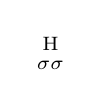
\begin{tikzpicture}[baseline=(current bounding box.center), scale=0.35,font=\scriptsize]% Adjust scale and font size as needed
        \node (H) at (0,0) {H};
        \node (sigma1) at (0,-0.8) {$\sigma\sigma$};
        %\node (sigma) at (0.25,-0.5){$\sigma$};
        %\draw[-] (H) -- (sigma);
    \end{tikzpicture}
}

\newcommand{\hlsyl}{
    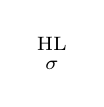
\begin{tikzpicture}[baseline=(current bounding box.center), scale=0.35,font=\scriptsize] % Adjust scale and font size as needed
        \node (H) at (0,0) {HL};
        \node (sigma1) at (0,-0.8) {$\sigma$};
        %\node (sigma) at (0.25,-0.5){$\sigma$};
        %\draw[-] (H) -- (sigma);
    \end{tikzpicture}
}

\newcommand{\hlhs}{
    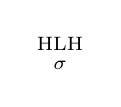
\begin{tikzpicture}[baseline=(current bounding box.center), scale=0.35,font=\scriptsize] % Adjust scale and font size as needed
        \node (H) at (0,0) {HLH};
        \node (sigma1) at (0,-0.8) {$\sigma$};
        %\node (sigma) at (0.25,-0.5){$\sigma$};
        %\draw[-] (H) -- (sigma);
    \end{tikzpicture}
}

\newcommand{\hlss}{
    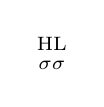
\begin{tikzpicture}[baseline=(current bounding box.center), scale=0.35,font=\scriptsize] % Adjust scale and font size as needed
        \node (H) at (0,0) {HL};
        \node (sigma1) at (0,-0.8) {$\sigma\sigma$};
        %\node (sigma) at (0.25,-0.5){$\sigma$};
        %\draw[-] (H) -- (sigma);
    \end{tikzpicture}
}

\newcommand{\hsl}{
    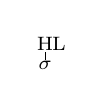
\begin{tikzpicture}[baseline=(current bounding box.center), scale=0.35,font=\scriptsize] % Adjust scale and font size as needed
        \node (H) at (0,0) {H};
        \node (L) at (0.5,0) {L};
        \node (sigma) at (0,-0.8) {$\sigma$};
        %\node (sigma) at (0.25,-0.5){$\sigma$};
        \draw[-] (H) -- (sigma);
    \end{tikzpicture}
}

\newcommand{\htones}{
    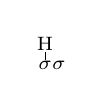
\begin{tikzpicture}[baseline=(current bounding box.center), scale=0.35,font=\scriptsize] % Adjust scale and font size as needed
        \node (H) at (0,0) {H};
        \node (sigma1) at (0,-0.8) {$\sigma$};
        \node (sigma2) at (0.5,-0.8){$\sigma$};
        \draw[-] (H) -- (sigma1);
    \end{tikzpicture}
}

\newcommand{\hsss}{
    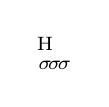
\begin{tikzpicture}[baseline=(current bounding box.center), scale=0.35,font=\scriptsize] % Adjust scale and font size as needed
        \node (H) at (0,0) {H};
        \node (sigma1) at (0,-0.8) {$\sigma$};
        \node (sigma2) at (0.35,-0.8){$\sigma$};
        \node (sigma3) at (0.7,-0.8){$\sigma$};
    \end{tikzpicture}
}


%\begin{document}
\begin{tikzpicture}[scale=0.6, font=\scriptsize]
    % Define nodes
    \node (41)  [red] at (-3,3)  {HLHL};
    \node (42)  [right of= 41, red]  {\hlhs};
    \node (43)  [right of= 42, red]  {\hlss};
    \node (44)  [right of= 43, red]  {\hsl};
    \node (45)  [right of= 44]  {\htones};
    \node (46)  [right of= 45] {\hsss};
    \node (31)  [below of= 42, red]  {HLH};
    \node (32)  [below of= 43, red] {\hlsyl};
    \node (33)  [below of= 44]{\htone};
    \node (34)  [right of= 33]  {\hsyll};
    \node (21)  [below of= 32, red]  {HL};
    \node (11)  [below right of= 21] {H};
    \node (22)  [above right of= 11]  {\h};
    \node (l)  [right of= 11] {L};
    \node (00)  [below of= l] {$\emptyset$};
    \node (sig)  [right of= l] {$\sigma$};
    \node(dots1)  [above of= sig] {...};
 % Box around node "HL"
 \node[draw, red, fit={(21)}, inner sep=0.05pt] {}; 
 
 % Small left arrow pointing to "G"
 \draw[red, ->] (21.west) -- ++(-0.5,0) node(G)[left] {\textit{G}};
 
 \node[left]  at (-4,3) {$k=4$};
 \node[left] at (-4,1.2) {$k=3$};
 \node[left] at (-4,-0.5) {$k=2$};
 \node[left] at(-4,-1.7) {$k=1$};
 \node[left] at (-4,-3.2) {$k=0$};    
     

    % Draw connections
    \draw (00) -- (l) ;
    \draw (00) -- (sig);
    \draw (00) -- (11);
    \draw (11) -- (21) -- (31);
    \draw (21) -- (32) -- (42);
    \draw (11) -- (22) -- (34) -- (46);
    \draw (22) -- (32) -- (43);
    \draw (22) -- (33) -- (44);
    \draw (22) -- (34) -- (45);
    \draw (31) -- (41);
    \draw (31) -- (42);
    \draw (32) -- (44);
    \draw (33) -- (45);

    
        % Add labels on the left

\end{tikzpicture}
%\end{document}

	\caption{Bottom-Up Learning over ARs}
	\label{fig:ARspace}
\end{figure}


As mentioned in Section 4.1, the algorithm starts its search from an empty structure. Two important functions are involved:  the \verb*|Contain| function checks for the presence of a given structure, and the \verb*|NextSupFact| function will generate its immediate superfactors. 

For each structure of size \(k\), its immediate superfactors will have a size of \(k+1\), and rank one level up higher in Figure \ref{fig:ARspace}. The one-step increase in size results from three potential changes: addition of a tone, or a TBU, or an association between the two tiers. As can be seen from Figure \ref{fig:ARspace}, when \(k=1\), the structure can be a floating H, a floating L, or a floating syllable. Take the floating H for instance, its superfactors (\(k=2\)) include a floating HL sequence, and a floating H with a floating syllable. If the HL sequence is found missing from the data \(D\), the algorithm will cease generating any superfactors and add HL into the grammar as a constraint forbidden by the language (labeled in red).

\todo[inline]{TG questioned the interpretation of ``floating''. If tone-TBU association can be seen as a feature, does the floating unit has (a) unspecified association feature, or (b) a negative association feature. If it is (a), then its superfactors include: an associated [H-$\sigma$] and also an unassociated [Hx$\sigma$]. Linguistically, the unassociated one could mean a ``delinking'' structure }

Two functions \verb*|NextSupFact| and \verb*|Contain| are essential parts the learner BUFIA infers grammars from. In the rest of the section, we will define these functions in terms of ARs.

\subsubsection{Contain} 
To illustrate Contain relation, I will follow the definition of \textit{restriction} and \textit{subfactor} given by \citet[p.94]{chandleeLearningPartiallyOrdered2019}.

\textbf{Definition 1.}\textit{ $A = \langle D^A; \lhd, R_A^1, \ldots, R_A^n \rangle$ is a restriction of $B = \langle D^B; \lhd, R_B^1, \ldots, R_B^n \rangle$ iff $D^A \subseteq D^B$ and for each $m$-ary relation $R_i$, we have $R_A^i = \{(x_1, \ldots, x_m) \in R_B^i \,|\, x_1, \ldots, x_m \in D^A\}$. }

Based on Definition 3, (\ref{ex:restr1}) is a restriction of (\ref{ex:restr2}) since $D^A = \{2,3,4,5\} \subseteq \{1,2,3,4,5\} = D^B$ and $R^A_H \in R^B_H, R^A_L \in R^B_L, R^A_\sigma \in R^B_\sigma, \lhd^A \in \lhd^B, \alpha^A \in \alpha^B$.

\begin{multicols}{2}
\ea \label{ex:restr1}
	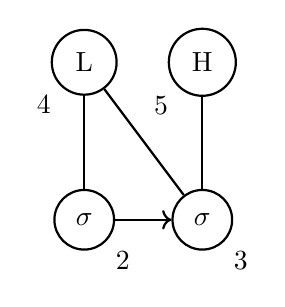
\begin{tikzpicture}
	%\node [state, label=below right:1] (s1) at (0,0) {$\sigma$};		
	\node [thick,state, label=below right:2] (s2) at (1.5,0) {$\sigma$};
	\node [thick,state, label=below right:3] (s3) at (3,0) {$\sigma$};
	%\node [state, label=below left:3] (t1) at (0,2) {H};
	\node [thick,state, label=below left:4] (t2) at (1.5,2) {L};
	\node [thick,state, label=below left:5] (t3) at (3,2) {H};
	%\draw [->] (t1) edge[above] node{\scriptsize{}} (t2);
	%\draw [->] (s1) edge[above] node{\scriptsize{}} (s2);
	\draw [thick,->] (s2) edge[above] node{\scriptsize{}} (s3);
	%\draw [-] (t1) edge[left] node{\scriptsize{}} (s1);
	%\draw [->] (t2) edge[above] node{\scriptsize{}} (t3);
	\draw [thick,-] (t2) edge[left] node{\scriptsize{}} (s2);
	\draw [thick,-] (t2) edge[left] node{\scriptsize{}} (s3);
	\draw [thick,-] (t3) edge[left] node{\scriptsize{}} (s3);
\end{tikzpicture}

\begin{minipage}{\linewidth}
	$\mathcal{M^A} = \{\mathcal{D} \mid R_H, R_L, R_\sigma, \lhd, \alpha \}$\\
	$\mathcal{D^A} = \{2, 3, 4, 5\}$\\
	$R^A_\sigma = \{2, 3\}$ \\
	$R^A_H = \{5\}$ \\
	$R^A_L = \{4\}$ \\
	$\lhd^A = \{\langle 2, 3\rangle \}$ \\
	$\alpha^A = \{\langle 2,4\rangle,  \langle 3, 5\rangle, \langle 4,2\rangle,  \langle 5,3\rangle \}$ 
\end{minipage}
\z
\end{multicols}

\begin{multicols}{2}
	\ea\label{ex:restr2}
	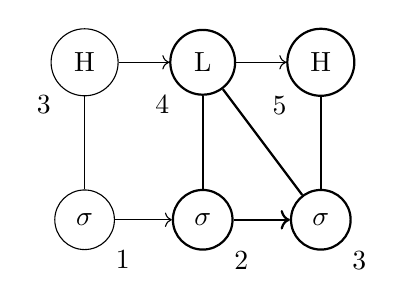
\begin{tikzpicture}
	\node [state, label=below right:1] (s1) at (0,0) {$\sigma$};			\node [thick,state, label=below right:2] (s2) at (1.5,0) {$\sigma$};
	\node [thick,state, label=below right:3] (s3) at (3,0) {$\sigma$};
	\node [state, label=below left:3] (t1) at (0,2) {H};
	\node [thick,state, label=below left:4] (t2) at (1.5,2) {L};
	\node [thick,state, label=below left:5] (t3) at (3,2) {H};
	\draw [->] (t1) edge[above] node{\scriptsize{}} (t2);
	\draw [->] (s1) edge[above] node{\scriptsize{}} (s2);
	\draw [thick,->] (s2) edge[above] node{\scriptsize{}} (s3);
	\draw [-] (t1) edge[left] node{\scriptsize{}} (s1);
	\draw [->] (t2) edge[above] node{\scriptsize{}} (t3);
	\draw [thick,-] (t2) edge[left] node{\scriptsize{}} (s2);
	\draw [thick,-] (t2) edge[left] node{\scriptsize{}} (s3);
	\draw [thick,-] (t3) edge[left] node{\scriptsize{}} (s3);
	\end{tikzpicture}

\begin{minipage}{\linewidth}
	$\mathcal{M^B} = \{\mathcal{D} \mid R_H, R_L, R_\sigma, \lhd, \alpha \}$\\
	$\mathcal{D^B} = \{1, 2, 3, 4, 5\}$\\
	$R^B_\sigma = \{1, 2, 3\}$ \\
	$R^B_H = \{3, 5\}$ \\
	$R^B_L = \{4\}$ \\
	$\lhd^B = \{\langle 1,2\rangle, \langle 2, 3\rangle,\langle 3,4\rangle, \langle4,5\rangle   \}$ \\
	$\alpha^B = \{\langle 1,3\rangle, \langle 2,4\rangle, \langle 3, 5\rangle, \langle 3,1\rangle, \langle 4,2\rangle, \langle 5,3\rangle  \}$ 
\end{minipage}
\z
\end{multicols}

With the concept of restriction, we can determine whether an AR $A$ is contained in another one $B$ by comparing \(A\) with a restriction of $B$, denotes as $B'$. If there exists a relation-preserving bijection between $A$ and $B'$, \(A\) is identified as a subfactor of $B$.

\textbf{Definition 2.} \textit{Structure $A$ is a subfactor of structure $B$ ($A \sqsubseteq B$) if $A$ is connected, there exists a restriction of $B$ denoted $B'$, and there exists $h:A \rightarrow B'$ such that for all $a_1, \ldots, a_m \in A$ and for all $R_i$ in the model signature: if $h(a_1), \ldots, h(a_m) \in B'$ and $R_i(a_1, \ldots, a_m)$ holds in $A$ then $R_i(h(a_1), \ldots, h(a_m))$ holds in $B'$. If $A \sqsubseteq B$, we also say that $B$ is a superfactor of $A$.}

In other words, if all relations held in \(A\) also hold in a related way in \(B\), \(A\) is considered as a subfactor of \(B\), and \(B\) is considered as a superfactor of \(A\). Figure (\ref{fig:superfactor}) illustrates the process of determining the containment relation between (\ref{fig:superfactor}a) and (\ref{fig:superfactor}c). One can identify (\ref{fig:superfactor}a) as a superfactor of (\ref{fig:superfactor}c) because there exists a restriction of (\ref{fig:superfactor}a) that has equivalent relations to those of (\ref{fig:superfactor}c).

\begin{figure}[ht]
	\centering
	% res.tex	
%\documentclass{standalone}
%\usepackage{tikz}
%\usetikzlibrary{fit} % Importing the fit library
%%%% This file is the preamble for the Pomona Linguistics Paper Template. 
%For stacking text, used here in autosegmental diagrams
\usepackage{stackengine}

%To combine rows in tables
\usepackage{multirow}
\usepackage{multicol}
\usepackage{enumitem}
\usepackage{subcaption}

%geometry helps manage margins, among other things.
\usepackage[margin =1in]{geometry}
\usepackage{tabularx}
%used to draw the bullet below
\usepackage{graphicx}

%Gives some extra formatting options, e.g. underlining/strikeout
\usepackage{ulem}

%For putting links into papers, also helps make cross-references in the paper smart references
\usepackage[colorlinks = true,
linkcolor = blue,
urlcolor  = blue,
citecolor = blue,
anchorcolor = blue]{hyperref} %smarter cross-references, these options turn links blue

%Use package/command below to create a double-spaced document, if you want one. Uncomment BOTH the package and the command (\doublespacing) to create a doublespaced document, or leave them as is to have a single-spaced document.
\usepackage{setspace}
\onehalfspacing

%paragraph formatting
\usepackage[parfill]{parskip}
\setlength{\parindent}{20pt}
\usepackage{titlesec}

%to position tables where I want
\usepackage{float}


%Basic math symbols 
\usepackage{pifont}
\usepackage{amssymb}
%\usepackage{nath}

%%%Gives shortcuts for glossing. The use of this package is NOT explained in the Quick Reference Guide, but the documentation is on CTAN for those that are interested. MJKD finds it handy for glossing. (https://ctan.org/pkg/leipzig?lang=en)
\usepackage{leipzig}

%Tables
\usepackage{caption} %For table captions
\usepackage{booktabs} %helps format tables

%For citations and bibliography - as of 9.1.2019 we don't explain citations in this Quick Reference Guide, but Pedro Martin's tutorial does (see links in the Guide).
\usepackage{natbib}

%Fonts
\usepackage{libertine}
\setmonofont[Scale=0.8]{Courier New Bold}
\usepackage{tipa}

%highlights text with \hl{text}
\usepackage{color, soul}

%%% 
% Customizing appearance of to-do notes
\usepackage[color=blue!20, bordercolor=blue]{todonotes}
\usepackage{algorithm}
\usepackage{algpseudocode}

\usepackage{verbatim} % for verbatim text
\usepackage{adjustbox} % for adjusting row height
\usepackage{array} % for centering text vertically in cells

%To combine rows in tables
\usepackage{multirow}
\usepackage{graphicx}
\usepackage{setspace}
%\doublespacing 


%Drawing Syntax Trees
\usepackage[linguistics]{forest}

%This specifies some formatting for the forest trees to make them nicer to look at
\forestset{
	asr/.style={
		for tree={
			align=center,
			parent anchor=south,
			%   child anchor=north,
			s sep=4mm,
			l sep=6mm
		}
	},
	strike/.style={
		edge label={
			node[midway, sloped, rotate=90] {=}
		}
	}
}

%These are useful for some of the details of arrows and other parts of syntax diagrams
\usetikzlibrary{positioning} %I've included this for the sake of making figures!
\usepackage{pstricks}
\usepackage{pst-node}



%% For numbered and glossed examples %%
\usepackage{gb4e}



\usepackage{tikz}

\newcommand{\circled}[1]{\begin{tikzpicture}[baseline=(word.base)]
	\node[draw, rounded corners, text height=8pt, text depth=2pt, inner sep=2pt, outer sep=0pt, use as bounding box] (word) {#1};
\end{tikzpicture}
}

\tikzset{
	state/.style={circle, draw, minimum size=20pt, inner sep=5pt}
}


%%%%%%%%%%%%%%%%%%%%%%%%%%%%%%%%%%%%%%%%%%%%%%%%%%%%%%%%%%%%
%%%%%%%%%%%%%%%%%%%%%%%%%%%%%%%%%%%%%%%%%%%%%%%%%%%%%%%%%%%%

% Useful Ling Shortcuts

\RequirePackage{leipzig}
%\RequirePackage{mathtools} % for \mathrlap

% % % Shortcuts  (borrowed from JZ, I'm still unsure exactly what xspace requires)
\RequirePackage{xspace}
\xspaceaddexceptions{]\}}

%This makes the \emptyset command be a nicer one
\let\oldemptyset\emptyset
\let\emptyset\varnothing
\newcommand{\nothing}{$\emptyset$}

%Not all of these are explained in the Quick Reference Guide, but they are here bc they are relevant to some of our students.
\newcommand{\1}{\rlap{$'$}\xspace}
\newcommand{\0}{\rlap{\textsuperscript{$ˆ{\circ}$}}\xspace}
\newcommand{\Lb}[1]{$\text{[}_{\text{#1}}$ } %A more convenient left bracket
\newcommand{\Rb}[1]{$\text{]}_{\text{#1}}$ } %A more convenient left bracket
\newcommand{\gap}{\underline{\hspace{1.2em}}}
\newcommand{\vP}{\emph{v}P}
\newcommand{\lilv}{\emph{v}}
\newcommand{\Abar}{A$'$-} %A more convenient A-bar notation
\newcommand{\ph}{$\varphi$\xspace} %A more convenient phi
\newcommand{\pro}{\emph{pro}\xspace}
\newcommand{\subs}[1]{\textsubscript{#1}} %A more convenient subscript
%\newcommand{\hd}{$^{\circ}$\xspace} %Symbol for printing head / degree symbol
\newcommand{\spells}{$\Longleftrightarrow$} %spellout arrow for morph spellout rules
\newcommand{\tr}[1]{\textit{t}\textsubscript{\textit{#1}}} %easy traces with subscript
\newcommand{\supers}[1]{\textsuperscript{#1}}
\newcommand{\type}[1]{\ensuremath{\langle{#1}\rangle}}% Type brackets for type-theory 	 ... \type{e,\type{s,t}}, from linguistics package			
\newcommand{\nl}{\ensuremath{\varnothing}}	  % =null; Null symbol ... \nl  (\null is already used) % Requires amssymb package, or a class that calls it %From Linguistics package

%This creates the command \bigcdot which is nice as a bullet for the conventional implicature formalism. Adapted from here: https://tex.stackexchange.com/questions/235118/making-a-thicker-cdot-for-dot-product-that-is-thinner-than-bullet
\makeatletter
\newcommand*\bigcdot{\mathpalette\bigcdot@{1}}
\newcommand*\bigcdot@[2]{\mathbin{\vcenter{\hbox{\scalebox{#2}{$\m@th#1\bullet$}}}}}
\makeatother



%%%%%%%%%%%%%%%%%%%%%%%%%%%%%%%%%%%%%%%%%%%%%%%%%%%%%%%%%%%%
%%%%%%%%%%%%%%%%%%%%%%%%%%%%%%%%%%%%%%%%%%%%%%%%%%%%%%%%%%%%

%A couple of packages that seemed to prefer being called toward the end of the preamble

%This package provides macros for typesetting SPE-style phonological rules.
\usepackage{phonrule}

%For using Greek letters outside of math mode.
\usepackage{textgreek}


%Random, lets us use the XeLaTeX logo. Not important to the template at all.
\usepackage{metalogo}

%The packages and tikz libraries below are used to generate the arrows on forest trees and linear diagrams that are explained in our Arrows explainer. https://www.overleaf.com/latex/templates/arrows-for-syntax-diagrams-with-forest/xjyvcszgcspv

\usetikzlibrary{positioning} %does something for the positioning of arrows and I can't remember what
\usetikzlibrary{arrows,arrows.meta} %gives extra details for arrows (specifically, the tips of arrows)
\usepackage{pstricks} %for horizontal arrows in linear diagrams
\usepackage{pst-node} %for placing nodes in horizontal arrow diagrams

\usepackage{forest}

%\begin{document}
	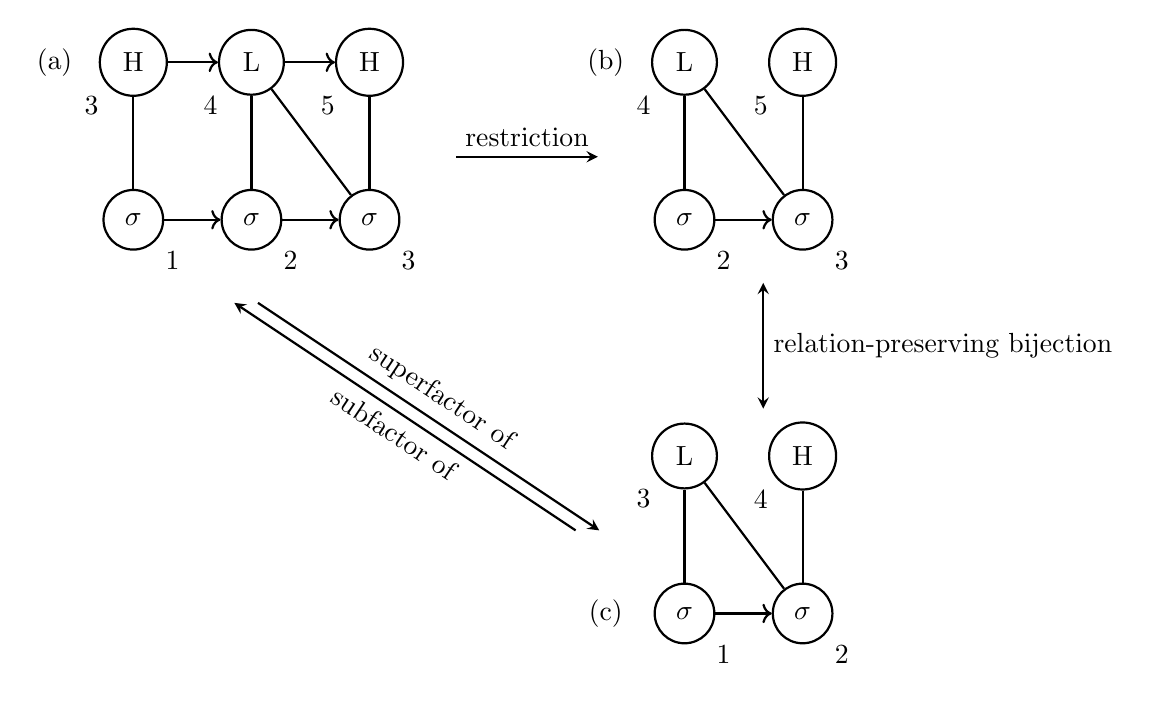
\begin{tikzpicture}[node distance=1.4cm, thick]
		% First figure \0
		\node [] (labela) at (-1,2) {(a)};
		\node [state, label=below right:1] (s1) at (0,0) {$\sigma$};
		\node [thick,state, label=below right:2] (s2) at (1.5,0) {$\sigma$};
		\node [thick,state, label=below right:3] (s3) at (3,0) {$\sigma$};
		\node [state, label=below left:3] (t1) at (0,2) {H};
		\node [thick,state, label=below left:4] (t2) at (1.5,2) {L};
		\node [thick,state, label=below left:5] (t3) at (3,2) {H};
		\draw [->] (t1) edge[above] node{\scriptsize{}} (t2);
		\draw [->] (s1) edge[above] node{\scriptsize{}} (s2);
		\draw [thick,->] (s2) edge[above] node{\scriptsize{}} (s3);
		\draw [-] (t1) edge[left] node{\scriptsize{}} (s1);
		\draw [->] (t2) edge[above] node{\scriptsize{}} (t3);
		\draw [thick,-] (t2) edge[left] node{\scriptsize{}} (s2);
		\draw [thick,-] (t2) edge[left] node{\scriptsize{}} (s3);
		\draw [thick,-] (t3) edge[left] node{\scriptsize{}} (s3);

		% Third figure
		\node [] (labelb) at (6,-5) {(c)};
		\node [thick,state, label=below right:1] (s2c) at (7,-5) {$\sigma$};
		\node [thick,state, label=below right:2] (s3c) at (8.5,-5) {$\sigma$};
		\node [thick,state, label=below left:3] (t2c) at (7,-3) {L};
		\node [thick,state, label=below left:4] (t3c) at (8.5,-3) {H};
		\draw [thick,->] (s2c) edge[above] node{\scriptsize{}} (s3c);
		\draw [thick,-] (t2c) edge[left] node{\scriptsize{}} (s2c);
		\draw [thick,-] (t2c) edge[left] node{\scriptsize{}} (s3c);
		\draw [thick,-] (t3c) edge[left] node{\scriptsize{}} (s3c);

		% Second figure
		\node [] (labelc) at (6,2) {(b)};
		\node [thick,state, label=below right:2] (s2b) at (7,0) {$\sigma$};
		\node [thick,state, label=below right:3] (s3b) at (8.5,0) {$\sigma$};
		\node [thick,state, label=below left:4] (t2b) at (7,2) {L};
		\node [thick,state, label=below left:5] (t3b) at (8.5,2) {H};
		\draw [thick,->] (s2b) edge[above] node{\scriptsize{}} (s3b);
		\draw [thick,-] (t2b) edge[left] node{\scriptsize{}} (s2b);
		\draw [thick,-] (t2b) edge[left] node{\scriptsize{}} (s3b);
		\draw [thick,-] (t3b) edge[left] node{\scriptsize{}} (s3b);
		
		% Arrows and labels
		\draw [shorten <=1mm, shorten >=1mm, ->, >=stealth, thick] (4,0.8) -- (6,0.8) node[midway, above] {restriction};
		\draw [shorten <=1mm, shorten >=1mm, <->, >=stealth, thick] (8,-0.7) -- (8,-2.5) node[midway, right] {relation-preserving bijection};
		\draw [shorten <=1mm, shorten >=1mm, ->, >=stealth, thick] (1.5,-1) -- (6,-4) node[midway, sloped, above] {superfactor of};
		\draw [shorten <=1mm, shorten >=1mm, <-, >=stealth, thick] (1.2,-1) -- (5.7,-4) node[midway, sloped, below] {subfactor of};
	\end{tikzpicture}
%\end{document}


	\caption{Superfactor, Restriction, and Subfactor AR}
	\label{fig:superfactor}
\end{figure}

Lastly, If $AR$ is the empty structure, it is contained by all $ARs$, but only contains itself. 

\subsubsection{Next Autosegmental Structure}
When the algorithm identifies the presence of a given structure, the \texttt{NextSupFac} function will generate its immediate superfactor. As mentioned in Section 4.2, the immediate superfactor of a structure of size \(k\) has a size of \( k+1 \), which can result from an one-unit addition of tone number \( t \), TBU numbers \( s \), or the number of associations \( \vert \alpha \vert \). In other words, an AR can be expanded using three operations: \texttt{addTone}, \texttt{addTBU}, or \texttt{addAssociation} depending on whether there are any floating units in the AR.\footnote{Theoretically, an association line can be formed between two non-floating units as long as it does not cross any other association lines, known as the No-Crossing Constraint \citep{goldsmith1976autosegmental, coleman1991no, hammond1988deriving}. In the current implementation, a new association will occur when there is at least one floating unit in the structure available to form an association. Since floating units are located on the rightmost side of the AR, at least one end of a new association line is at the rightmost end of the tonal string or the TBU string. This also ensures that all constraints of size less than $k$ will be considered.}

\[
\texttt{NextSupFact(AR)} =
\begin{cases}
	\texttt{addTone(AR)} \cup \texttt{addTBU(AR)} & \text{if } \texttt{containFloat(AR) = False} \\
	\texttt{addTone(AR)} \cup \texttt{addTBU(AR)} \cup \texttt{addAssociation(AR)} & \text{if } \texttt{containFloat(AR) = True}
\end{cases}
\]

First, the function \texttt{containFloat} checks for the presence of a floating unit in the AR. For AR = $\{D\mid R_H, R_L, R_\sigma, R_\lhd, R_\alpha\}$, a unary relation \(R_i \in \{R_H, R_L, R_\sigma\}\) is considered \textit{floating} if \(R_i \in  R_\lhd \wedge R_i \notin R_\alpha\). The two cases are shown in (\ref{ar:ftt}) and (\ref{ar:fts}). AR (\ref{ar:ftt}) contains a floating tone L at position \{4\}. This element is in a successor relation of \{$\langle 3,4 \rangle$\}  on the tonal tier but missing from the association relation, which only contain one pair \{$\langle 1,2 \rangle$\}. Similarly, AR (\ref{ar:fts}) contains a floating syllable at position \{2\} for it is present in the successor relation \{$\langle 1,2 \rangle$\} but absent from the association relation \{$\langle 1,3 \rangle, \langle 1,4 \rangle$\}.

\begin{multicols}{2}
	\ea AR containing a floating tone \label{ar:ftt}
	
	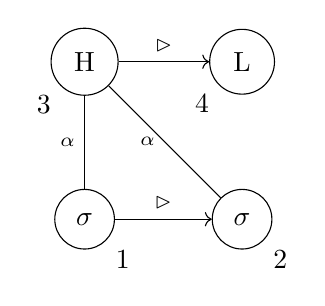
\begin{tikzpicture} 
		\node [state, label=below right:1] (s1) at (0,0) {$\sigma$};
		\node [state, label=below right:2] (s2) at (2,0) {$\sigma$};
		%\node [state, label=below right:3] (s3) at (4,0) {$\sigma$};
		\node [state, label=below left:3] (t1) at (0,2) {H};
		\node [state, label=below left:4] (t2) at (2,2) {L};
		\draw [->] (t1) edge[above] node{\scriptsize{$\vartriangleright$}} (t2);
		\draw [->] (s1) edge[above] node{\scriptsize{$\vartriangleright$}} (s2);
		%\draw [->] (t1) edge[above] node{\scriptsize{$\vartriangleright$}} (s3);
		\draw [-] (t1) edge[left] node{\scriptsize{$\alpha$}} (s1);
		\draw [-] (t1) edge[left] node{\scriptsize{$\alpha$}} (s2);
		%\draw [-] (t2) edge[left] node{\scriptsize{$\alpha$}} (s3);
	\end{tikzpicture}
	\z
	\ea AR containing a floating syllable   \label{ar:fts}
	
	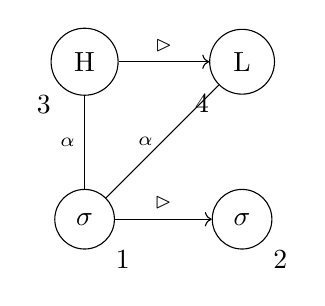
\begin{tikzpicture} 
	\node [state, label=below right:1] (s1) at (0,0) {$\sigma$};
	\node [state, label=below right:2] (s2) at (2,0) {$\sigma$};
	%\node [state, label=below right:3] (s3) at (4,0) {$\sigma$};
	\node [state, label=below left:3] (t1) at (0,2) {H};
	\node [state, label=below left:4] (t2) at (2,2) {L};
	\draw [->] (t1) edge[above] node{\scriptsize{$\vartriangleright$}} (t2);
	\draw [->] (s1) edge[above] node{\scriptsize{$\vartriangleright$}} (s2);
	%\draw [->] (t1) edge[above] node{\scriptsize{$\vartriangleright$}} (s3);
	\draw [-] (t1) edge[left] node{\scriptsize{$\alpha$}} (s1);
	\draw [-] (t2) edge[left] node{\scriptsize{$\alpha$}} (s1);
	%\draw [-] (t2) edge[left] node{\scriptsize{$\alpha$}} (s3);
	\end{tikzpicture}
	\z
\end{multicols}


The \verb*|addTone| function is defined as follows: for any autosegmental representation \(AR\) with a size of \(k\) and a string \(w = t_1t_2\ldots t_n, t \in \{H,L\}\) on the tonal tier, there exists one and only one \(AR'\), which is \(AR\)'s \(k+1\) expansion on the tonal tier if \(AR'\) has a tonal string \(w' = wt_{n-1}\). From a model-theoretic perspective, for an AR with a model signature of $M = \{D\mid R_H, R_L, R_\sigma, R_\lhd, R_\alpha\}$, \(R_i\) is denoted as the final\todo{do i need to define ``final''} element in the tonal string, \(i \in D,\text{ and }R_i \in \{R_H,R_L\}\). Then \(AR\)'s \(k+1\) expansion on the tonal tier will only change its domain and unary relation \(D' = D \cup i+1, R_i \in R_H \implies R_{i+1} \in R_L \wedge R_i \in R_L \implies R_{i+1} \in R_H\). In other words, a tonal string can only be expanded by adding one tone unit at a time, which is the opposite tone unit of the original final tone. 


The \verb*|addTBU| function is defined as for any autosegmental representation \(AR\) with a size of \(k\) and has a length of $s$ on the TBU tier, there exists one and only one \(AR'\), which is \(AR\)'s \(k+1\) expansion on the TBU tier if \(AR'\) has a TBU length of $s+1$. In terms of model signature, \(D' = D \cup i+1, R_{i+1} \in R_\sigma\).

\begin{multicols}{2}
	\ea  Add a New tone
	
	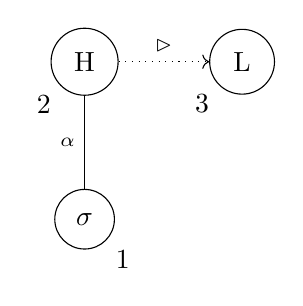
\begin{tikzpicture}
		\node [state, label=below right:1] (s1) at (0,0) {$\sigma$};
		\node [state, label=below left:2] (t1) at (0,2) {H};
		\node [state, label=below left:3] (t2) at (2,2) {L};
		\draw [->, dotted] (t1) edge[above] node{\scriptsize{$\vartriangleright$}} (t2);
		\draw [-] (t1) edge[left] node{\scriptsize{$\alpha$}} (s1);
	\end{tikzpicture}
	\z
	\ea  Add new TBU
	
	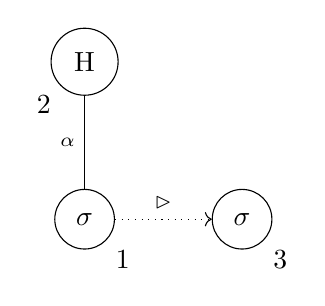
\begin{tikzpicture} 
	\node [state, label=below right:1] (s1) at (0,0) {$\sigma$};
	\node [state, label=below right:3] (s2) at (2,0) {$\sigma$};
	\node [state, label=below left:2] (t1) at (0,2) {H};
	\draw [->, dotted] (s1) edge[above] node{\scriptsize{$\vartriangleright$}} (s2);
	\draw [-] (t1) edge[left] node{\scriptsize{$\alpha$}} (s1);
\end{tikzpicture}
	\z
\end{multicols}


The \verb*|addAssociation| function will only apply to those ARs containing floating units. A new association $(i,j)$ is only considered formed validly if and only if there does not exist an association  $(i',j') \in R_\alpha$ such that $(i' > i \wedge j' < j) \vee (i' < i \wedge j' > j)$. This rule is enforced in accordance to the No-Crossing Rule in Autosegmental Theory \citep{goldsmith1976autosegmental,coleman1991no,hammond1988deriving}. In this case, there are 3 ways to form possible new associations: the floating tone connects to the syllable as in (\ref{ft2cs}); the floating syllable connects to the tone as in (\ref{fs2ct}); the floating tone connects to a floating syllable as in (\ref{ft2fs}).
\\
\begin{multicols}{3}
	\ea \label{ft2cs}
	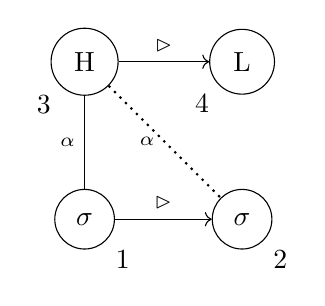
\begin{tikzpicture} 
		\node [state, label=below right:1] (s1) at (0,0) {$\sigma$};
		\node [state, label=below right:2] (s2) at (2,0) {$\sigma$};
		\node [state, label=below left:3] (t1) at (0,2) {H};
		\node [state, label=below left:4] (t2) at (2,2) {L};
		\draw [->] (t1) edge[above] node{\scriptsize{$\vartriangleright$}} (t2);
		\draw [->] (s1) edge[above] node{\scriptsize{$\vartriangleright$}} (s2);
		\draw [-] (t1) edge[left] node{\scriptsize{$\alpha$}} (s1);
		\draw [thick, dotted] (t1) edge[left] node{\scriptsize{$\alpha$}} (s2);
	\end{tikzpicture}
	\z
	\ea	\label{fs2ct}
	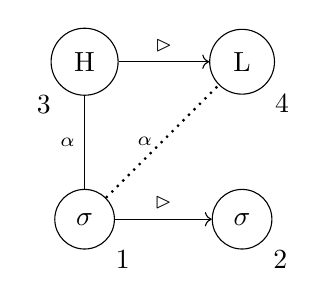
\begin{tikzpicture} 
		\node [state, label=below right:1] (s1) at (0,0) {$\sigma$};
		\node [state, label=below right:2] (s2) at (2,0) {$\sigma$};
		\node [state, label=below left:3] (t1) at (0,2) {H};
		\node [state, label=below right:4] (t2) at (2,2) {L};
		\draw [->] (t1) edge[above] node{\scriptsize{$\vartriangleright$}} (t2);
		\draw [->] (s1) edge[above] node{\scriptsize{$\vartriangleright$}} (s2);
		\draw [-] (t1) edge[left] node{\scriptsize{$\alpha$}} (s1);
		\draw [thick, dotted] (s1) edge[left] node{\scriptsize{$\alpha$}} (t2);
	\end{tikzpicture}
	\z
	\ea \label{ft2fs}
	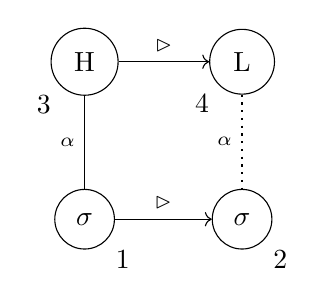
\begin{tikzpicture} 
		\node [state, label=below right:1] (s1) at (0,0) {$\sigma$};
		\node [state, label=below right:2] (s2) at (2,0) {$\sigma$};
		\node [state, label=below left:3] (t1) at (0,2) {H};
		\node [state, label=below left:4] (t2) at (2,2) {L};
		\draw [->] (t1) edge[above] node{\scriptsize{$\vartriangleright$}} (t2);
		\draw [->] (s1) edge[above] node{\scriptsize{$\vartriangleright$}} (s2);
		\draw [-] (t1) edge[left] node{\scriptsize{$\alpha$}} (s1);
		\draw [thick, dotted] (t2) edge[left] node{\scriptsize{$\alpha$}} (s2);
	\end{tikzpicture}
	\z
\end{multicols}

\section{Case Study: Hausa}
This section presents a case study of using BUFIA to identify tonotactic constraints over autosegmental representations in Hausa, a language with two contrast tones (H and L) spoken in West Africa. It demonstrates tonotactic patterns can be learned successfully over ARs given a certain length on the syllable tier \(s\) and length on the tonal tier \(t\). Out of 664 words represented as strings extracted from the Hausa database, which include nonborrowed and unanalyzable words translated into ARs, the learning algorithm successfully identified 7 AR constraints (\(s\leq3\) and \(t\leq3\)). This case study illustrates the feasibility and efficiency of learning over autosegmental representations. First, tonal learning over autosegmental representations significantly reduces the hypothesis space: of all 664 words, only 
26 distinct AR patterns were found, effectively making the positive dataset smaller. Secondly, the algorithm exhibits three advantages compared to previous literature: it discovers previously identified constraints, provides more accurate and specific constraints than ones posited previously which are found to be too general, and discovers new constraints that have not been reported yet. This section first reviews the basic tonology of Hausa then introduces the three major steps of the experiment: data extraction, representation conversion, and algorithm implementation. The results will be discussed in the Section 6.\footnote{Source codes can be accessed from \href{https://github.com/lihan829/AR_learning.git}{https://github.com/lihan829/AR\_learning.git}}

\subsection{Tonology of Hausa}
Let us first review the basic tonology of the language in question. Hausa has a 2-tone system (H and L) and the tone-bearing unit is the syllable which consists of at most two moras. A falling contour (HL) can be formed when the two tones occupy a single syllable. There is no monosyllabic LH or any three-tone contours. According to Newman's reference grammar of Hausa, the tonal patterns are summarized as a \textbf{right-to-left} spreading phenomenon \citep[p.600]{Newmanbook}.
\begin{quote}
	``If a word has more tones than syllables, then two tones can dock on the same syllable if that syllable has the necessary weight (i.e. two moras) to carry the two tones. The tones of the melody are assigned to the syllables from right to left. If there are more syllables than tones, one keeps on spreading the tone in a leftward fashion...If there are more tones than syllables, then one assigns the tones from right to left until one has run out of syllables, whereupon one assigns the remaining tone to the initial syllable (assuming that it is a bimoraic syllable that can carry two tones)." 
\end{quote}

Newman argues that the leftward spreading pattern explains that, for nonderived canonical words with the contour tone, the HL contour is typically formed on the last syllable. In disyllabic words, common patterns include HL, LH, and HH; whereas in trisyllabic words, common patterns are HLH, LHL, HHL, and LHH. The LL sequence is uncommon across all instances, whether LL, HLL, or LLL. \cite{zoll2003optimal} argues the analysis of directional spreading leads to paradoxical outputs (e.g. *HLL,*LLH but LHH, HHL) and therefore proposes instead a quality-based perspective. According to Zoll, the constraint LAPSE (L-tone spreading to two syllables) overranks CLASH (H-tone spreading to two syllables). The absence of LL, particularly at the word final position, has also been explained as a Low Tone Raising rule \phonb{L}{H}{L}{\#} first proposed by \cite{Leben}. In summary, the tonotactic patterns attested in Hausa for canonical nonderived words are listed below in the format of constraints.

\ea Linguistically Attested Constraints in Hausa:
\begin{enumerate}
	\item *LH: No monosyllabic rising
	\item *(3$\mu$): No three-tone contour
	\item NF-Cont: No initial HL contour for di-/polysyllabic words
	\item *LL: Avoid LL sequence
\end{enumerate}
\z 

The learning problem is whether these tonal constraints can be accurately captured by an algorithm. The 
hypothesis in the current paper is: if the hypothesis space for the learning algorithm comprises all possible ARs (under a certain size) that a language can generate, and these ARs are represented over model-theoretic representations, then the bottom-up learner will successfully capture the tonotactic grammar by searching from the most generalized AR to more specific ones against the positive data. If the algorithm can generate a set of constraints in Hausa, how do they correspond to previously identified linguistic constraints? Driven by these questions, a case study of Hausa tonotactic patterns was designed.

\subsection{Data Preparation}
The data used for the current experiment comes from Hausa dataset \citep{wold-4} from The World Loanword Database (WOLD) \citep{wold}. The WOLD includes 41 languages. Each language dateset consist of around 1460 core words with meanings in the Loanword Typology (LWT) meaning list.  For the Hausa dataset, the vocabulary contains 1668 core meaning-word pairs. The dataset includes information such as ``Form", ``Meaning", ``Borrowed", ``Likelihood", ``Analyzability", ``Age", and ``Source". The fields most relevant to the current study are listed in Table \ref{tab:fields}. To get the canonical tonal patterns in Hausa, only those words that were clearly not borrowed from other languages and were simple monomorphemic words were used. All others were filtered out. A total of 664 words transcribed in orthography remained and stored in a .cvs file.


\begin{table}[H]
	\centering
	\begin{tabular}{c|>{\arraybackslash}m{0.65\textwidth}|>{\arraybackslash}m{0.15\textwidth}}
		\hline
		\multicolumn{1}{c|}{\textbf{Field}} & \multicolumn{1}{c|}{\textbf{Explanation}} & \multicolumn{1}{c}{\textbf{Example}}  \\
		\hline
		Form  & Transcription in orthography where á = H tone, à = L tone, âa = F tone, and double vowels indicate long vowels  &  ƙásáa \\
		\hline
		Meaning & The meaning of the form as listed in the Loanword Typology (LWT) list & ``the land" \\
		\hline
		Borrowed & Four levels of borrowing certainty ranging from 0 (``no evidence of borrowing") to 1 (``clearly borrowed") & no evidence for borrowing\\
		\hline
		Analyzability & Describes the degree of analyzability of a word form, ranging from ``Unanalyzable'' (monomorphemic word) to ``Analyzable phrasal" (verb-noun phrases or prep-noun phrases) & unanalyzable\\
		\hline
	\end{tabular}
	\caption{Description of fields relevant to the current study}
	\label{tab:fields}
\end{table}


\subsection{Representation Conversion}

Since the goal is to apply the algorithm to autosegmental representations, a Python code was created to convert all string representations into ARs. These ARs are stored as tuples, as illustrated in the \textit{Coding} column of Table \ref{tab:conversion}. Each tuple contains two pieces of information: the tonal melody of the word (e.g., \texttt{'H'} or \texttt{'HLH'}) and a list of pairs indicating associations of tones and tone-bearing units (e.g., \verb|[(1,1),(1,2)]|.

 Within the association list, the first element $i$ in each pair $(i,j)$ specifies the index of the tone and the second element $j$ specifies the syllable index. In other words, $(i,j)$ indicates that tone $i$ is associated with syllable $j$. The list orders the associations from the first tone to the last, and also the first syllable to the last syllable. Thus from the last pair in the list $(i_n,j_n)$, one can easily infer that the current AR structure contains $i_n$ tone unit(s) and $j_n$ syllable(s).

Take the word \textit{ƙásáa} for instance, the AR is represented as \verb|('H'[(1,1),(1,2)])| in the coding system. This reads as the melody the AR bears has one tone \texttt{'H'}, and has an association of \verb|[(1,1),(1,2)]|. More specifically, \verb|(1,1)| indicates the first tone \texttt{'H'} connects to the first syllable and \verb|(1,2)| means the first tone `H' again connects to the second syllable. For the word containing contour tones such as \textit{bâutáa}, the AR shows a tone of \texttt{'HLH'} and an association of \verb|[(1,1),(2,1),(3,2)]| which means first two tone units HL both connects to the first syllable while the last third tone H connects to the second syllable. The entire AR contains 3 tones and 2 syllables.

After converting and eliminating identical ARs, 26 distinct ARs were identified from among 664 string representations (See Attachment \ref{apx:ar}). The given data shows a maximum syllable number is 5, indicating the non-borrowed monomorphemic words in Hausa are likely within a 5-syllable length. Besides, there are 8 melodic patterns found in the data, which are H, L, LH, HL, LHL, HLH, HLHL, LHLH.
\begin{table}[ht]
	\centering
	\begin{tabular}{c|>{\centering \arraybackslash}m{0.3\textwidth}|>{\centering\arraybackslash}m{0.3\textwidth}}
	\hline
	\textbf{Transcription} & \textbf{AR} &\textbf{Coding}\\
	%\multicolumn{1}{c|}{\textbf{Transcription}} & \multicolumn{1}{c|}{\textbf{AR}} & \multicolumn{1}{c}{\textbf{Coding}}  \\
	\hline
		\textit{ƙásáa} & \adjustbox{valign=c,height=0.09\textwidth}{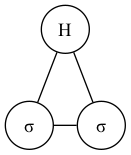
\includegraphics{figs/ƙásáa}} & \texttt{('H'[(1,1),(1,2)])} \\
		\hline
		\textit{bâutáa} & \adjustbox{valign=c,height=0.08\textwidth}{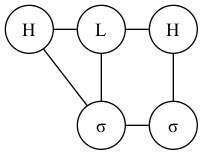
\includegraphics{figs/bâutáa}} & \texttt{('HLH',[(1,1),(2,1),(3,2)])} \\
		\hline
	\end{tabular}
	\caption{Corresponding Strings, ARs, and Coding}
	\label{tab:conversion}
\end{table}

\subsection{Implementing BUFIA over ARs}
After converting all string representations into ARs, the next step is to run BUFIA on the dataset of 26 attested ARs. Since BUFIA initiates from the empty structure, it generates its immediate superfactors: a floating H, a floating L, and a floating syllable. These floating units are indicated by \verb*|None| in the list. In Table \ref{tab:float}, AR1 and AR2 contain a floating tone and a floating syllable respectively and both have \verb*|None| in their coding. AR (\ref{floattone}) has \verb*|(2,None)| in its association list, indicating that the second tone is not connected to any syllable; AR (\ref{floatsyl}) has \verb*|(None,2)| indicating that the second syllable is not connected to any tone.
\begin{table}[H]
\begin{tabular}{ c|c|c} % Adjust column widths as needed
\hline
\textbf{floating tone} &	\textbf{floating syllable} &	\textbf{float tone and syllable} \\ \hline
	\begin{subfigure}{0.29\textwidth}
		\centering
		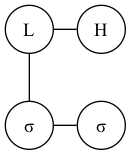
\includegraphics[width=0.52\textwidth]{figs/LH}			\caption{\texttt{(LH,[(1,1),(2,None)])}}	
		\label{floattone}
	\end{subfigure} & 
	\begin{subfigure}{0.29\textwidth}
		\centering
		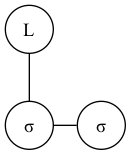
\includegraphics[width=0.52\textwidth]{figs/L}
		\caption{\texttt{(L,[(1,1),(None,2)])}}
		\label{floatsyl}			
	\end{subfigure} &
	\begin{subfigure}{0.33\textwidth}
		\centering
		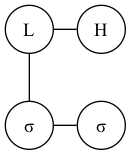
\includegraphics[width=0.49\textwidth]{figs/float}
		\caption{\texttt{(LH,[(1,1),(None,2),(2,None)])}}
		\label{floatsyl}			
	\end{subfigure} \\
\hline
\end{tabular}
\caption{Coding for ARs with float units}
\label{tab:float}
\end{table}


\section{Results and Discussion}

The algorithm BUFIA discovered 7 tonotactic constraints missing from the data when the syllable sizes $s$ is no greater than 3 and the tone sizes $t$ is no greater than 3. In Table \ref{tab:cons}, cells with 0 indicates that no constraints were found at current $s$ and $t$ sizes; cells with a dash indicates no new constraints were added on the basis of the previous sizes. In the following section, I will compare the linguistically attested constraints (will be referred as ``rule constraints'') with the algorithm detected constraints (will be referred as ``BUFIA constraints'') and discuss whether the two match and, if not, what would be the gap between the two.

\begin{table}[H]
	\centering
	\renewcommand{\arraystretch}{2} % Adjust the value (e.g., 1.5) to increase or decrease the height of thex rows
	\begin{tabular}{c|>{\centering\arraybackslash}m{0.1\textwidth}|>{\centering\arraybackslash}m{0.15\textwidth}|>{\centering\arraybackslash}m{0.52\textwidth}}
		\hline
		& $t = 1$ & $t= 2$ & $t = 3$ \\
		\hline
		$s = 1$ & 0 
				&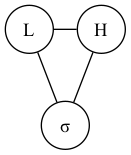
\includegraphics[width=0.12\columnwidth]{hausacons/0LHt2s1}
				& - \\
				
\hline				
		$s = 2$ & 0 
				&			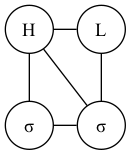
\includegraphics[width=0.12\columnwidth]{hausacons/1HLt2s2} 		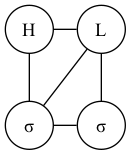
\includegraphics[width=0.12\columnwidth]{hausacons/2HLt2s2}
				& -\\
\hline

		$s = 3$ &	0 %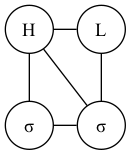
\includegraphics[width=0.19\columnwidth]{hausacons/cons1}
				&	- %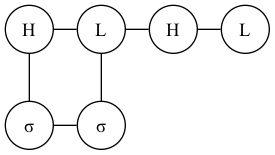
\includegraphics[width=0.21\columnwidth]{hausacons/cons3} 
				&	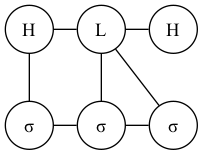
\includegraphics[width=0.19\columnwidth]{hausacons/3HLHt3s3} 	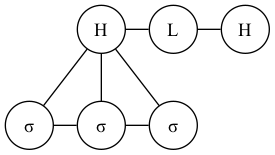
\includegraphics[width=0.25\columnwidth]{hausacons/4HLHt3s3} 
				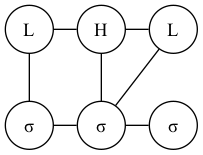
\includegraphics[width=0.21\columnwidth]{hausacons/5LHLt3s3}
				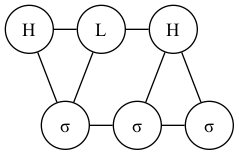
\includegraphics[width=0.24\columnwidth]{hausacons/6HLHt3s3}  
				%	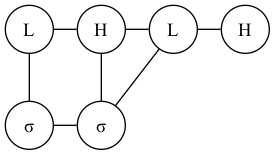
\includegraphics[width=0.18\columnwidth]{hausacons/cons8}\\						
			
			
	\end{tabular}
	\caption{Constraints over AR in Hausa when $s \leq 3,   t \leq 3$}
	\label{tab:cons}
\end{table}


Table \ref{tab:monoarcons} lists both Rule Constraint 1 and 2, and a BUFIA constraint concerning monosyllabic forms. Rule Constraint 1 states that the language forbids monosyllabic LH and Constraint 2 states no 3-tone contour, which are translated into an AR fashion where no LH, LHL, and HLH are linked to a single syllable. One can see that the algorithm effectively identified the absence of monosyllabic rising tone when \( s=1 \) and \( t=2 \) since (\ref{cons1a}) and (\ref{cons1d}) are identical. Moreover, since both (\ref{cons1b}) and (\ref{cons1c}) contain (\ref{cons1a}/\ref{cons1d}) as a subfactor, forbidding (\ref{cons1a}/\ref{cons1d}) automatically entails forbidding both three-tone superfactors. Consequently, the algorithm has already identified (\ref{cons1d}) as a constraint, and therefore ceased further generating or checking its superfactors. In conclusion, we can consider the algorithm accurately captures the monosyllabic tonal patterns.

\begin{table}[H] 
	\centering
	%\renewcommand{\arraystretch}{1} % Adjust the value (e.g., 1.5) to increase or decrease the height of the rows
	\begin{tabular}{c|c}
		\hline
		Rule Constraints & BUFIA Constraints\\
		\hline
		\begin{subfigure}{0.13\columnwidth}
			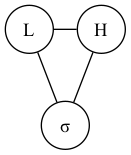
\includegraphics[width=\textwidth]{hausacons/cons0}
			\caption{}
			\label{cons1a}
		\end{subfigure}
		\begin{subfigure}{0.2\columnwidth}
			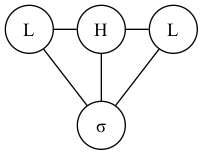
\includegraphics[width=\textwidth]{graph/LHL1}
			\caption{}
			\label{cons1b}
		\end{subfigure}
		\begin{subfigure}{0.2\columnwidth}
			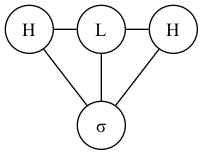
\includegraphics[width=\textwidth]{graph/HLH1}
			\caption{}
			\label{cons1c}
		\end{subfigure} &   
		\begin{subfigure}{0.13\columnwidth}
			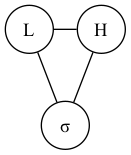
\includegraphics[width=\textwidth]{hausacons/cons0}
			\caption{}
			\label{cons1d}
		\end{subfigure}  \\
		\hline
	\end{tabular}
	\caption{Linguistically Attested and BUFIA Detected ARs for monosyllabic words}
	\label{tab:monoarcons}
\end{table}


\textbf{Constraint 3} bans initial HL contours for di/polysyllabic nonderived words, which can be depicted as the Rule Constraint (\ref{cons3a}) in Table \ref{tab:disyl}. In this case, edge markers are added to indicate the word initial position. The graph indicates that when the word has $\geq$ 2 syllables, a structure which has HL on its initial syllable will be forbidden in Hausa. An extra syllable following the first one in (\ref{cons3a}) is important since Hausa does allow a monosyllabic word with HL (e.g. \textit{mâi} ``oil'', \textit{kâi} ``head'' ). 

\begin{table}[ht]	
	\centering
	%\renewcommand{\arraystretch}{1} % Adjust the value (e.g., 1.5) to increase or decrease the height of the rows
	\begin{tabular}{c|c}
		\hline
		Rule Constraint & 	BUFIA Constraint \\
		\hline
		\begin{subfigure}{0.24\textwidth}
			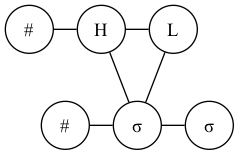
\includegraphics[width=\textwidth]{figs/HLinitial.png}
			\caption{}
			\label{cons3a}
		\end{subfigure} &
		\begin{subfigure}{0.137\textwidth}
			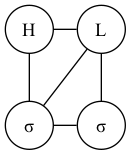
\includegraphics[width=\textwidth]{hausacons/cons2}
			\caption{}
			\label{cons3b}
		\end{subfigure}
		\begin{subfigure}{0.25\textwidth}
			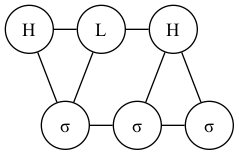
\includegraphics[width=\textwidth]{hausacons/6HLHt3s3}
			\caption{}
			\label{cons3c}
		\end{subfigure}\\
		\hline
	\end{tabular}
	\caption{Rule constraints and BUFIA constraints concerning initial HL}
	\label{tab:disyl}
\end{table}



Two constraint ARs (\ref{cons3b}) and  (\ref{cons3c}) are found by BUFIA. It should be mentioned the syllables in (\ref{cons3b}) and  (\ref{cons3c}) are not position-specified: the leftmost syllable in the both graphs does not necessarily correspond to the first syllable in the word. In other words, not only these AR constraints themselves but also stuctures containing them will be banned. Now we will consider (\ref{cons3b}) and  (\ref{cons3c}) in the most generalized case where they are viewed as word initially and comparable to (8a).\footnote{This is admittedly a limitation of the current experiment. Thanks to Thomas Graf for pointing this out, where edge markers should have been considered to obtain a more generalized constraint without any assumption of possible positions where contour tones can be formed. The reasons that the current experiment does not consider the word-internal contours are: (1) in the traditional Autosegmental Theory, contour tones form as a result of one-to-one, left-to-right association conventions that govern the mapping of tonal melody, which leads to contour forms usually at word-final position \citep{goldsmith1976autosegmental}; (2) In African languages, contours demonstrate an ``edge effect'' and largely limited to the final tone-bearing unit of the domain \citep{yip1989contour} and Hausa contour distribution shows the same pattern \citep{Newmanbook}; (3) even in languages where tonal melodies are not justified, contours still tend to prefer a prosodic final position, as argued by \cite{zhang2009contour}, which is attributed to the longer duration of these syllables.}
	

The first one (\ref{cons3b}) is in a disyllabic form and states that no AR has been found to contain at least two syllables where the first one is associated with a HL contour and the second one with a L tone. The second one (\ref{cons3c}) reads that no AR has been found to have at least 3 syllables where the first one is associated with a HL contour and the rest two are linked with a H. Obviously, this indicates structures that contain (8a) but do not contain (8b-c) are present in the current data. We can list out the superfactors of (8a) and exclude those contain (8b-c) to find out the missing gaps between the Rule constraints and BUFIA constraints, which are listed as (\ref{missing1},\ref{missing2}) below.

\begin{multicols}{2}
\ea Disyllabic form with initial HL: $\check{\sigma}\acute{\sigma}$

	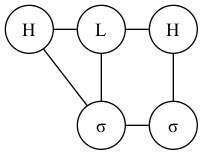
\includegraphics[width=0.25\textwidth]{hausacons/missing}
	\label{missing1}
\z

\ea Trisyllabic form with initial HL: $\check{\sigma}\acute{\sigma}\grave{\sigma}$

	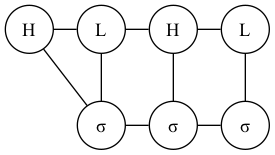
\includegraphics[width=0.36\textwidth]{hausacons/missing2}
	\label{missing2}
\z
\end{multicols}

Via a reverse search, 7 words were found to match these two structures, as shown in Ex (\ref{hlhwords}). This result show that the Rule Constraint of initial HL needs to be made more explicit and restricted if it aims to account for all data. 
\ea Hausa words do contain an initial HL

\label{hlhwords}
\begin{tabular}{ll}
	ƙyânwáa &	``the cat'' \\
	kûnnée 	& 	``the ear''\\
	tsûmmáa	& 	``the handkerchief or rag''\\
	sâiwáa	& 	``the root''\\
	jînƙái	& 	``the pity''\\
	bâutáa 	&	``to worship, to obey''\\
	yânyáawàa & ``the fox (fennec of Sahara)''
\end{tabular}
\z


\textbf{Constraint 4} states the avoidance of LL sequences. It is worth noting that this is not a strict ban. \citet[p.606]{Newmanbook} pointed out LL exceptions are ``relatively uncommon and mostly represent identifiable or presumed loanwords''. Correspondingly, the algorithm did not report any constraint when \(t=1\) and \(s =2\), confirming there are cases (as in (\ref{LL})) where disyllabic words containing LL sequences. By examining 4 words containing LL sequence in our dataset, it is easy to notice that many of them belong to the question words, which could contribute to the LL exceptional cases. 
\ea \label{LL}
\begin{tabular}{ll}
	màcè & ``female''\\
	yàayàa & ``how''\\
	yàushè & ``when'' \\
	wànè & ``which'' \\
\end{tabular}
\z

Additionally, although it has been commonly reported that the trisyllabic HLL and LLH are disfavored in Hausa \citep{zoll2003optimal,Leben,Newmanbook} the BUFIA constraint (\ref{bufiaHLLH}) indicates that both patterns are actually present in the current data. In fact, the LLH pattern is not uncommon: 16 words were found to bear the same tonal melody with the same association (see Appendix \ref{LLHnHLL}). Moreover, from (\ref{bufiaHLLH}), we can revise the ``no LL spreading'' rule to: LL spreading is banned when two L-toned syllables are wedged between two H-toned syllables.\footnote{To be more precise, the BUFIA constraint (\ref{bufiaHLLH}) states that no L tone can occupy two adjacent syllables and is simultaneously wedged between one H-toned syllable and another H tone whose association does not have to be specified. Theoretically, the second H tone could be linked to the rightmost syllable that L tone spreads onto or linked to a fourth syllable by itself. However, the first option is not available since LH cannot dock on the same syllable.}

\begin{table}[ht]
	\centering
	\begin{tabular}{c|c}
		\hline
			Rule Constraint  & BUFIA Constraint \\
		\hline
		\begin{subfigure}{0.19\textwidth}
			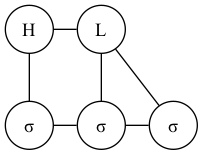
\includegraphics[width=\textwidth]{hausacons/HLL.png}
			\caption{}
			\label{consHLL}
		\end{subfigure}
		\begin{subfigure}{0.19\textwidth}
			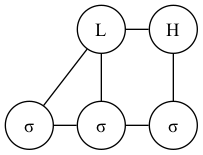
\includegraphics[width=\textwidth]{hausacons/LLH}
			\caption{}
			\label{consLLH}
		\end{subfigure}&
		\begin{subfigure}{0.19\textwidth}
		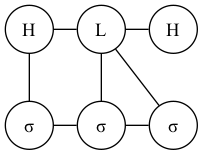
\includegraphics[width=\textwidth]{hausacons/3HLHt3s3}
		\caption{}
		\label{bufiaHLLH}
		\end{subfigure} 	\\	
 		\hline
	\end{tabular}
	\caption{Linguistically Predicted and BUFIA Detected ARs for HLL and LLH patterns}
	\label{tab:llh}
\end{table}



In summary, this section reports the results of implementing BUFIA to find tonotactic patterns over ARs and compares computationally attested constraints with linguistically reported constraints. It is found that a bottom-up learning algorithm can effectively learn tonotactic patterns over autosegmental representations. Additionally, three outcomes emerge regarding the matching between BUFIA constraints and Rule constraints. First, the two coincide, indicating that BUFIA accurately captures exactly what previous linguistic rules formalize. Second, BUFIA constraints are more restrictive and specific than linguistic constraints without overgeneralizing the patterns. Lastly, the algorithm also uncovers some patterns, usually of a larger size, that have not been reported in any other literature.

\section{Conclusion} 
This paper shows the first attempt to learn tonotactic patterns over autosegmental representations using a bottom-up learning algorithm. Through a case study of Hausa, 26 distinct ARs among 654 surface-true Hausa words were found, and tonotactic constraint grammar consist of 14 ARs ($\leq$ 4 syllables and 3 tones). Furthermore, by comparing BUFIA constraints and Rule constraints, we found sometimes the two matches but more often BUFIA constraints were more explicit or specific than the Rule constraints. For example, we found patterns that were identified to be constraints occur in the positive data, which is due to the constraint only applies during certain phonological contexts. We also found patterns that haven not reported by previous linguistic analysis, which perhaps due to the structure's growing size. These results show the feasibility of tonotactic grammar inference over autosegmental representations and extends the advantaged of using algorithm to enhance previous generalization.

However, this paper does not provide any comparison between learning results using string representations and ARs, which is a limitation and also a reasonable next step to take. Comparing the efficiency of the same algorithm learning over two types of representations would be more convincing in determining whether tonotactic patterns should be better learned over ARs.


\todo{Questions below were asked by Thomas, Ellen}
Additionally, the scope of this paper only reaches tonotactic patterns. There are studies on learning tonal processes using Autosegmental Input Strictly Local functions \citep{chandlee2019autosegmental,zhu2020extending}, which delve deeper into the mapping between underlying forms to surface forms. It would be interesting to see how specific tonal processes could be captured by the algorithm implementation. \todo[inline]{TG asked - any way to track the derivative and notderivative tones (eg F tone as an underlying tone vs. HL combination). I dont think i answered the question at all...}

Lastly, one major point of this paper is to demonstrate the autonomous nature of tones can be learned as a bistring which connects a vocal folds configuration to the linear timing system. Building upon the findings of this study, one may ask whether and how autosegmental learning can benefit Asian language research such as Mandarin or Cantonese. Different from the African systems, tonal languages in Asia usually have a richer tonal inventory, including tones at different levels and several contour tones. Additionally, these languages usually do not have rich morphology like African languages. In particular, Cantonese and Mandarin are to a large extent seen as syllable-tone languages where each syllable has a specified underlying tone, and all syllables in a word retain the underlying tone when combined \citep{yip2002tone}. In this specific case, learning over ARs specifically for tonotactic patterns may not significantly reduce the hypothesis space since there is no restriction on either tier of ARs. However, for languages rich in sandhi processes and showing interactions between tone and segments or other phonation features, representations that separate tone from other features may be worth investigating to see any better results.


\appendix
\section{Hausa Autosegmental Structures}\label{apx:ar}
\begin{table}[H]
	\centering
	\begin{tabular}{ccccl}
		\hline
		\textbf{No.} &\textbf{Tone Number} & \textbf{Syllable Number} & \textbf{Tonal Melody} & \textbf{Association} \\
		\hline
	1	&1 & 1 & H & [(1, 1)] \\
	2	&1 & 1 & L & [(1, 1)] \\
	3	&1 & 2 & H & [(1, 1), (1, 2)] \\
	4	&1 & 2 & L & [(1, 1), (1, 2)] \\
	5	&1 & 3 & H & [(1, 1), (1, 2), (1, 3)] \\
	6	&1 & 4 & H & [(1, 1), (1, 2), (1, 3), (1, 4)] \\
	7&	2 & 1 & HL & [(1, 1), (2, 1)] \\
8	&	2 & 2 & LH & [(1, 1), (2, 2)] \\
9	&	2 & 2 & HL & [(1, 1), (2, 2)] \\
10	&	2 & 3 & LH & [(1, 1), (2, 2), (2, 3)] \\
11	&	2 & 3 & LH & [(1, 1), (1, 2), (2, 3)] \\
12	&	2 & 3 & HL & [(1, 1), (1, 2), (2, 3)] \\
13	&	2 & 3 & HL & [(1, 1), (2, 2), (2, 3)] \\
14	&	2 & 4 & LH & [(1, 1), (1, 2), (1, 3), (2, 4)] \\
15	&	2 & 4 & HL & [(1, 1), (1, 2), (1, 3), (2, 4)] \\
16	&	2 & 4 & LH & [(1, 1), (2, 2), (2, 3), (2, 4)] \\
17	&	2 & 5 & HL & [(1, 1), (1, 2), (1, 3), (1, 4), (2, 5)] \\
18	&	3 & 2 & LHL & [(1, 1), (2, 2), (3, 2)] \\
19	&	3 & 2 & HLH & [(1, 1), (2, 1), (3, 2)] \\
20	&	3 & 3 & LHL & [(1, 1), (2, 2), (3, 3)] \\
21	&	3 & 3 & HLH & [(1, 1), (2, 2), (3, 3)] \\
22	&	3 & 4 & LHL & [(1, 1), (2, 2), (2, 3), (3, 4)] \\
23	&	3 & 4 & HLH & [(1, 1), (1, 2), (2, 3), (3, 4)] \\
24	&	3 & 5 & LHL & [(1, 1), (1, 2), (1, 3), (2, 4), (3, 5)] \\
25	&	4 & 3 & HLHL & [(1, 1), (2, 1), (3, 2), (4, 3)] \\
26	&	4 & 4 & LHLH & [(1, 1), (2, 2), (3, 3), (4, 4)] \\
		\hline
	\end{tabular}
	\caption{26 distinct ARs among 655 Hausa core word list}
	\label{tab:patterns}
\end{table}

\section{Hausa Constraints}
\begin{table}[H]
	\centering
	\begin{tabular}{ccccl}
		\hline
		No & t & s & Melody & Association \\
		\hline
1	&	1 & 4 & L & (1, 1), (1, 2), (1, 3), (1, 4) \\
2	&	2 & 1 & LH & (1, 1), (2, 1) \\
3	&	2 & 2 & HL & (1, 1), (1, 2), (2, 2) \\
4	&	2 & 2 & HL & (1, 1), (2, 1), (2, 2) \\
5	&	2 & 4 & HL & (1, 1), (2, 1), (None, 2), (None, 3), (None, 4) \\
6	&	2 & 4 & HL & (1, 1), (2, 2), (2, 3), (None, 4) \\
7	&	2 & 4 & LH & (1, 1), (1, 2), (2, 3), (2, 4) \\
8	&	2 & 4 & LH & (1, 1), (1, 2), (2, None), (1, 3), (1, 4) \\
9	&	3 & 3 & HLH & (1, 1), (2, 2), (2, 3), (3, None) \\
10	&	3 & 3 & HLH & (1, 1), (1, 2), (2, None), (1, 3), (3, None) \\
11	&	3 & 3 & LHL & (1, 1), (2, 2), (3, 2), (None, 3) \\
12	&	3 & 3 & HLH & (1, 1), (2, 1), (3, 2), (3, 3) \\
13	&	3 & 4 & HLH & (1, 1), (1, 2), (2, None), (1, 3), (3, None), (None, 4) \\
14	&	3 & 4 & HLH & (1, 1), (2, 2), (3, 3), (3, 4) \\
15	&	3 & 4 & HLH & (1, 1), (1, 2), (2, 3), (3, None), (2, 4) \\
16	&	3 & 4 & HLH & (1, 1), (1, 2), (2, None), (1, 3), (3, None), (1, 4) \\
17	&	3 & 4 & LHL & (1, 1), (2, 2), (2, 3), (3, None), (2, 4) \\
18	&	3 & 4 & LHL & (1, 1), (1, 2), (2, 3), (3, None), (2, 4) \\
19	&	3 & 4 & LHL & (1, 1), (1, 2), (2, None), (1, 3), (3, None), (1, 4) \\
20	&	4 & 2 & HLHL & (1, 1), (2, 2), (3, None), (4, None) \\
21	&	4 & 2 & HLHL & (1, 1), (1, 2), (2, None), (3, None), (4, None) \\
22	&	4 & 2 & LHLH & (1, 1), (1, 2), (2, None), (3, None), (4, None) \\
23	&	4 & 2 & LHLH & (1, 1), (2, 2), (3, 2), (4, None) \\
24	&	4 & 2 & HLHL & (1, 1), (2, 1), (3, 2), (4, 2) \\
25	&	4 & 3 & LHLH & (1, 1), (2, 2), (2, 3), (3, None), (4, None) \\
26	&	4 & 4 & HLHL & (1, None), (None, 1), (2, None), (None, 2), (3, None), (None, 3), (4, None), (None, 4) \\
		\hline
	\end{tabular}
	\caption{26 tonotactic constraints in autosegmental representations in Hausa}
	\label{tab:hausaar}
\end{table}

\section{LLH and HLL patterns in Hausa}
\begin{table}[H]
	\centering
	\begin{tabular}{c|l}
		\hline
		\textbf{Form} & \textbf{Meaning} \\
		\hline
		tàuràaróo & ``the star" \\
		tùnkùyáu & ``the flea" \\
		\textbf{shànshàaníi} & ``the centipede" \\
		màƙèesúu & ``the firefly" \\
		\textbf{zàzzàɓíi} & ``the fever" \\
		\textbf{ƙàiƙàyíi} & ``the itch" \\
		màlàfáa & ``the hat or cap" \\
		gìzàagóo & ``the adze" \\
		màràicée & ``the evening" \\
		jùuyàayíi & ``the anxiety" \\
		\textbf{gùngùníi} & ``to mumble" \\
		shùugàbáa & ``the president" \\
		tàbàráu & ``the spectacles/glasses" \\
		tùrùríi & ``the steam" \\
		sùrùkái & ``the parents-in-law" \\
		ƙwàràngwál & ``the carcass" \\
		sábòodà & ``because" \\
		\hline
	\end{tabular}
	\caption{Hausa Words with either LLH or HLL pattern}
	\label{tab:hausawords}
\end{table}


%%%%%%%%%%%%%%%%%%%%%%%%%%%%%%%%%%%
\bibliography{refs.bib}
\bibliographystyle{apalike}
\end{document}